\section{\thesection.~A Data-Driven History of Tonality}

% \againframe<{5,7}>{disciplines}

% \begin{frame}{\insertsectionhead}
%   Motivation / Questions
% \end{frame}

\againframe<7->{corpus_pipeline}

\subsection{1. Recovering the line of fifths}

\begin{frame}{\insertsectionhead}
    \onslide<3->{
    \begin{center}
    \resizebox{.75\textwidth}{!}{
      % colors for line of fifths
\definecolor{Gb}{HTML}{6d6dff}
\definecolor{Db}{HTML}{8585ff}
\definecolor{Ab}{HTML}{9d9dff}
\definecolor{Eb}{HTML}{b5b5ff}
\definecolor{Bb}{HTML}{cdcdff}
\definecolor{F}{HTML}{e5e5ff}
\definecolor{C}{HTML}{fffdfd}
\definecolor{G}{HTML}{ffe5e5}
\definecolor{D}{HTML}{ffcdcd}
\definecolor{A}{HTML}{ffb5b5}
\definecolor{E}{HTML}{ff9d9d}
\definecolor{B}{HTML}{ff8585}
\definecolor{Fs}{HTML}{ff6d6d}

% draw picture
\begin{tikzpicture}[scale=2]

\draw[latex-latex] (-3.5,0) -- (3.5,0) ; % line

% down ticks
\foreach \x/\label in  {-6/G$\flat$,
                         -5/D$\flat$,
                         -4/A$\flat$,
                         -3/E$\flat$,
                         -2/B$\flat$,
                         -1/F,
                         0/C,
                         1/G,
                         2/D,
                         3/A,
                         4/E,
                         5/B,
                         6/F$\sharp$}
\draw[shift={(\x/2,0)},color=black] (0pt,0pt) -- (0pt,-5pt) node[below] {\label};
% % up ticks
% \foreach \x in  {-6,...,6}
% \draw[shift={(\x/2,0)},color=black] (0pt,0pt) -- (0pt,5pt) node[above] {$\x$};

% draw circles
\foreach \x/\color in {-6/Gb,
                         -5/Db,
                         -4/Ab,
                         -3/Eb,
                         -2/Bb,
                         -1/F,
                         0/C,
                         1/G,
                         2/D,
                         3/A,
                         4/E,
                         5/B,
                         6/Fs}
  \node [circle, fill=\color,scale=1.5, draw=black] (\x) at (\x/2,0) {};

\end{tikzpicture}
}
    \end{center}
  }

  \begin{figure}
    \onslide<2->{
    \begin{subfigure}[c]{.48\linewidth}
      \centering
      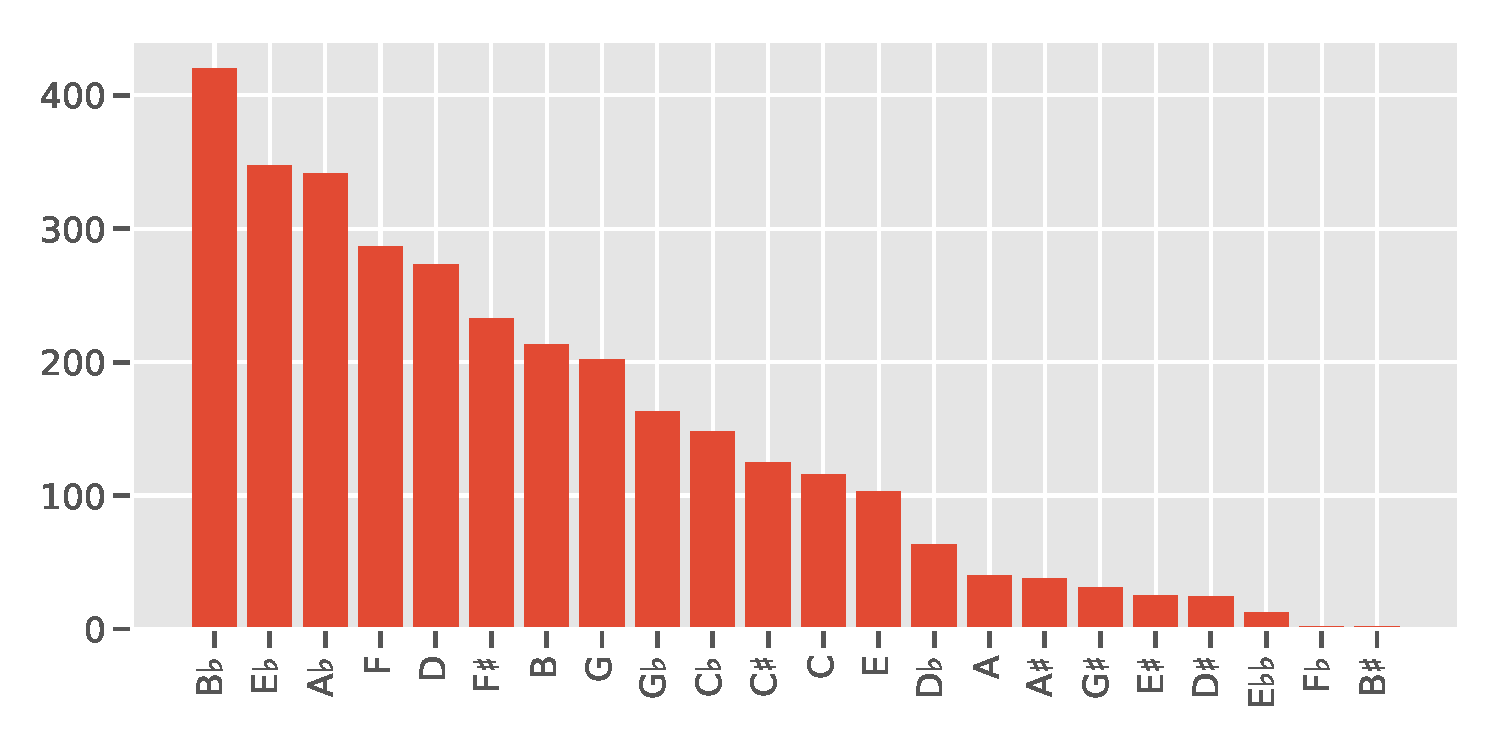
\includegraphics[width=\textwidth]{img/tpc_dists_sorted.pdf}
      \subcaption{Ranked note frequencies.}
    \end{subfigure}
    }
    \hfill
    \onslide<4->{
    \begin{subfigure}[c]{.48\linewidth}
      \centering
      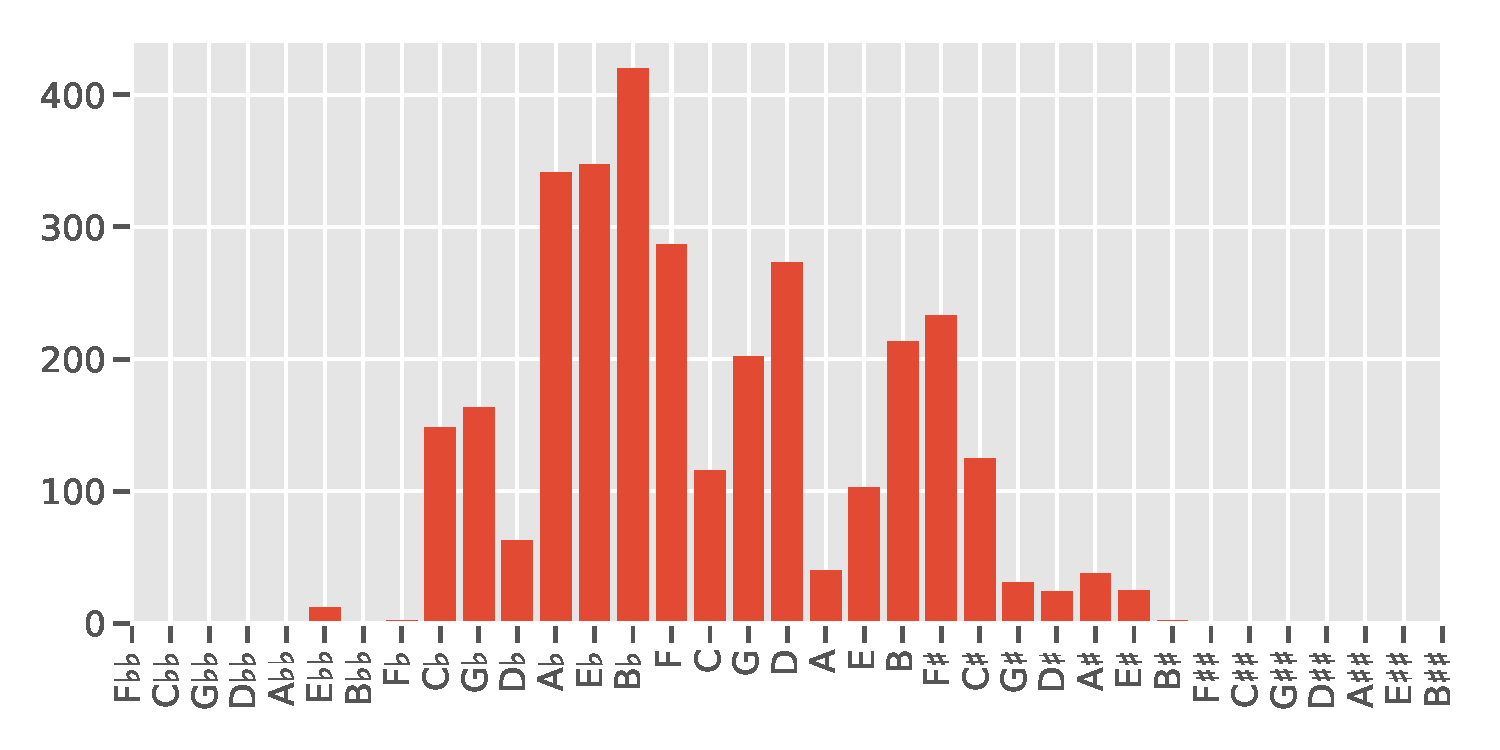
\includegraphics[width=\textwidth]{img/tpc_dists.pdf}
      \subcaption{Note frequencies on line of fifths.}
    \end{subfigure}
    }
    \caption{F. Schubert, \emph{Impromptu}, op.~90/2 in E$\flat$~major.}
    \label{}
  \end{figure}
\end{frame}

\note[itemize]{
  \item Using Music Theory: arranging on LoF shows structure
  \item define fifth width
  \item FW >= 7: chromaticism; FW >= 12: enharmonicism
}

\begin{frame}{\insertsectionhead}

  Corpus studies allow us to
  \begin{itemize}
    \item widen the \alert{scope} to entire collections of pieces
    \item empirically \alert{test} the validity of music-theoretical concepts
  \end{itemize}

  \pause

  $\Rightarrow$ Is the line of fifths \emph{really} a \alert{relevant structure} for pitch-class distributions?

  \pause

  \begin{enumerate}[\color{epflred}1.]
    \item Gather a large corpus.
    \item Transform pieces to pitch-class distributions.
    \item Apply \emph{dimensionality reduction} to uncover underlying structures.
  \end{enumerate}
\end{frame}

\begin{frame}{\insertsectionhead}

  \begin{columns}
    \begin{column}{.3\textwidth}
      % Sources
      % \begin{itemize}
      %   \item existing published \& accessible data
      %   \item web search
      %   \item transcription
      % \end{itemize}
      % Dataset \citep{Moss2020}
      The corpus:
      \begin{itemize}
        \item 2,012 pieces
        \item 75 composers
        \item approx. 600 years
      \end{itemize}
    \end{column}
    %
    \begin{column}{.7\textwidth}
      \begin{figure}
        \centering
        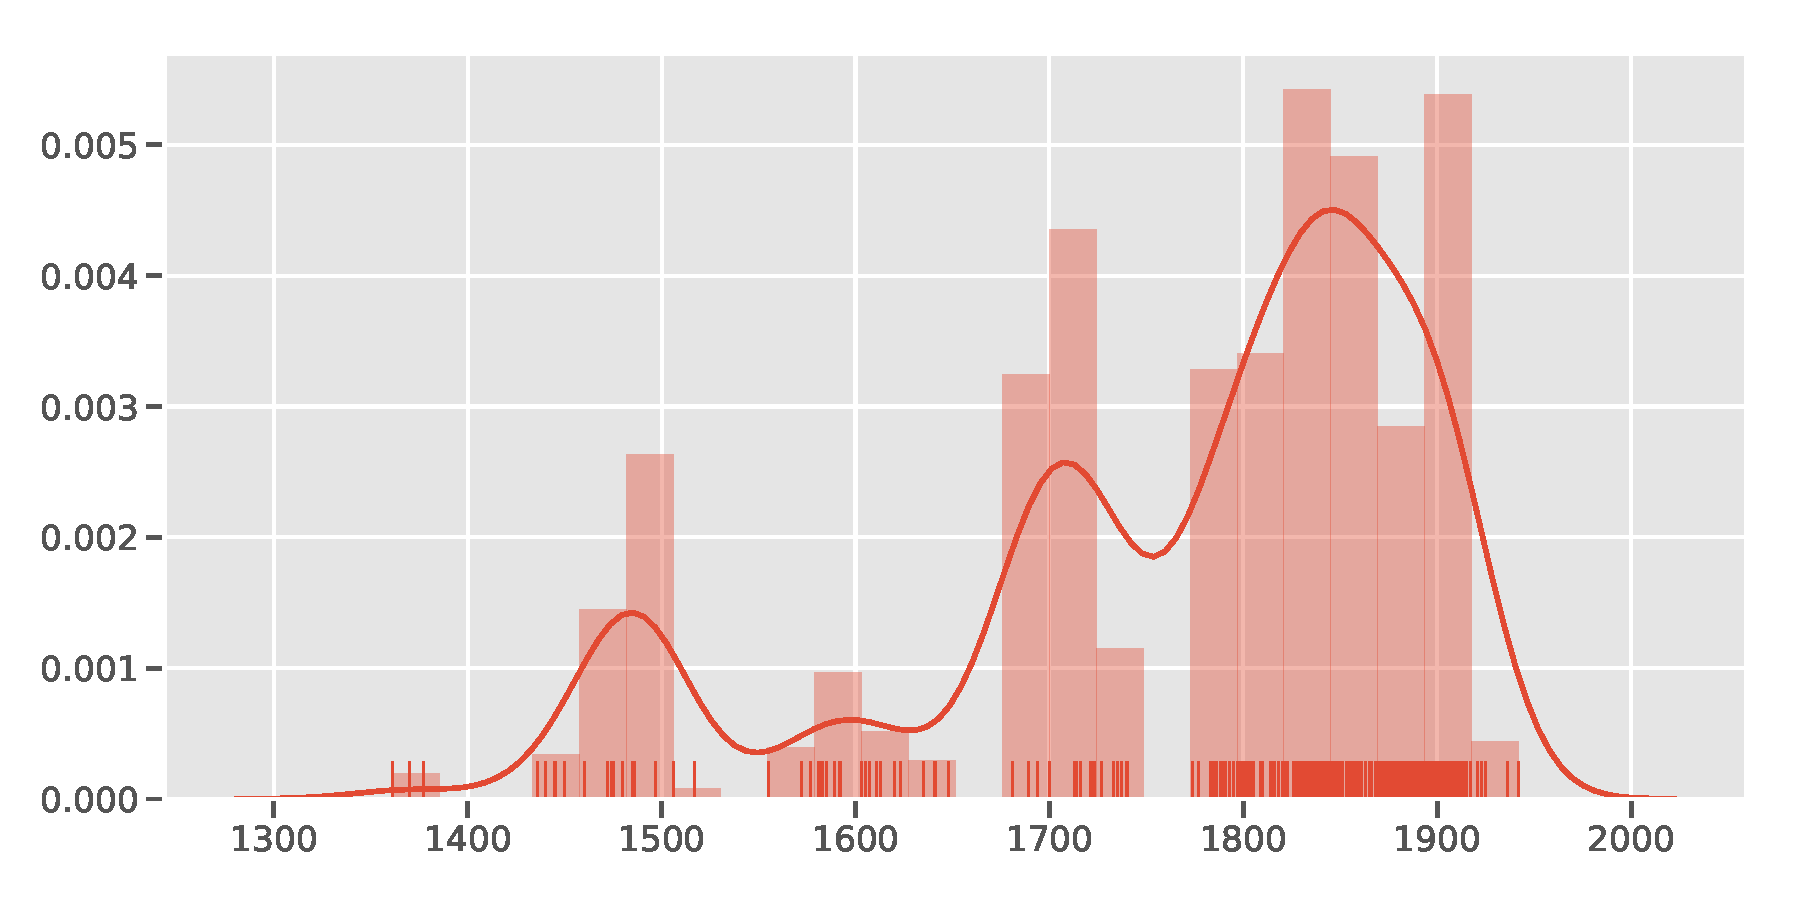
\includegraphics[width=\textwidth]{img/piece_dist.pdf}
        \caption{Historical distribution of the corpus.}
        \label{}
      \end{figure}
    \end{column}
  \end{columns}
\end{frame}

\begin{frame}{\insertsectionhead}
  \begin{figure}
  \captionsetup[subfigure]{justification=centering}
    \onslide<2->{
      \begin{subfigure}[t]{.3\textwidth}
        \centering
        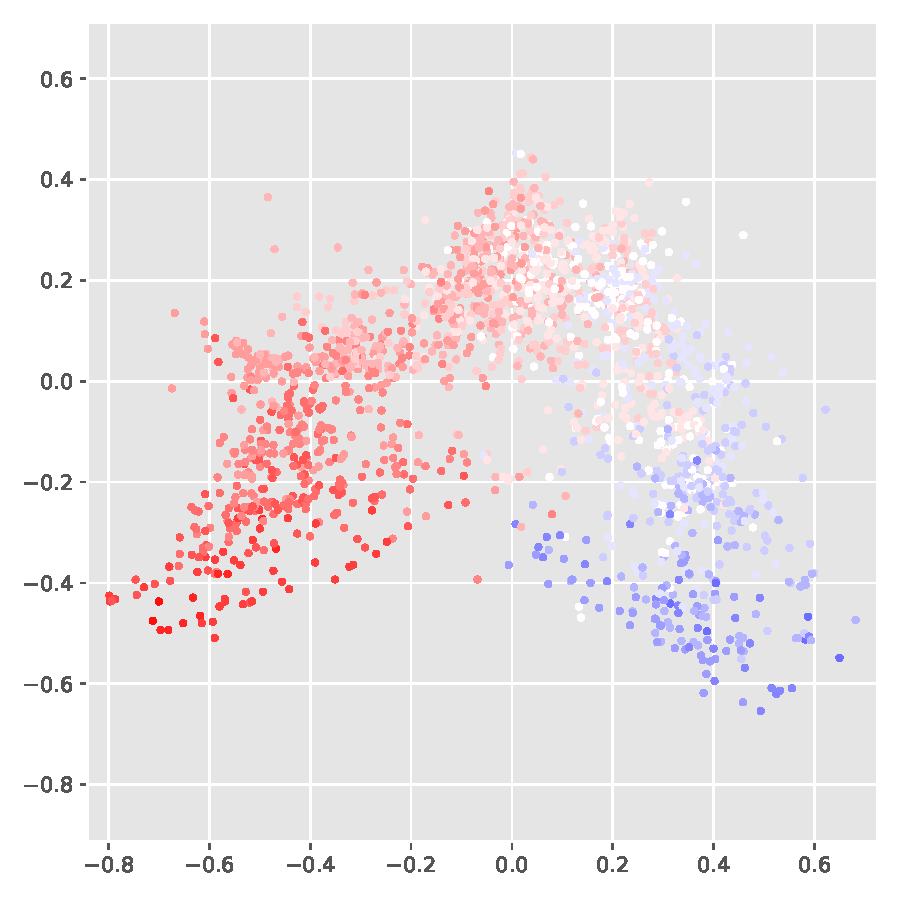
\includegraphics[width=\linewidth]{img/dim_reduct_Isomap.pdf}
        \subcaption*{Isomap.}
      \end{subfigure}
    }
    \hfill
    \onslide<1->{
      \begin{subfigure}[t]{.3\textwidth}
        \centering
        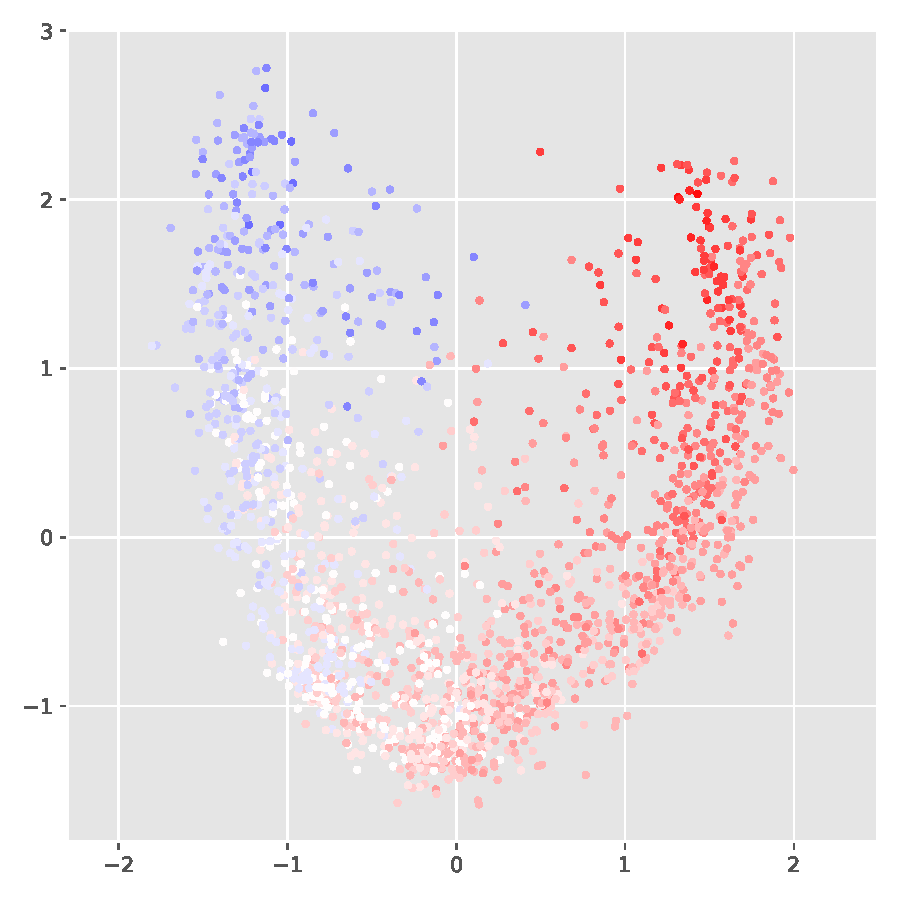
\includegraphics[width=\linewidth]{img/dim_reduct_PCA.pdf}
        \subcaption*{Principal Component Analysis.}
      \end{subfigure}
    }
    \hfill
    \onslide<2->{
    \begin{subfigure}[t]{.3\textwidth}
      \centering
      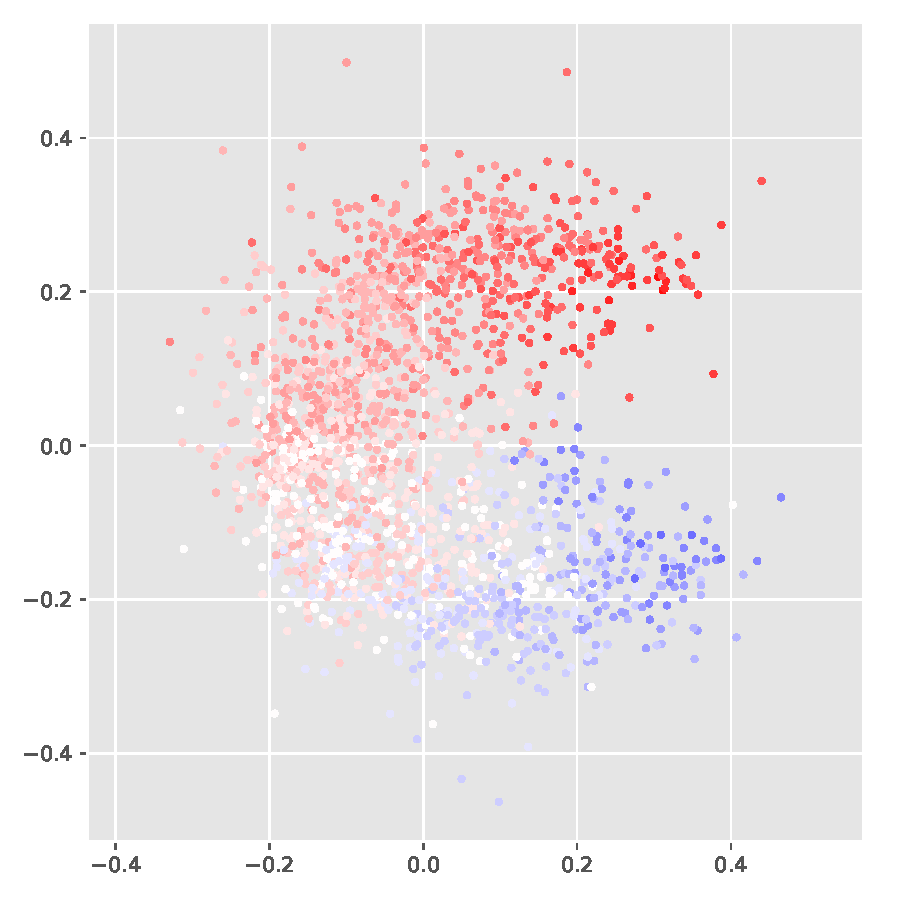
\includegraphics[width=\linewidth]{img/dim_reduct_MDS.pdf}
      \subcaption*{Multi-Dimensional Scaling.}
    \end{subfigure}
    }
    \caption{Dimensionality reduction of tonal space.}
    \label{}
  \end{figure}

  \onslide<1->{
    \begin{center}
    \resizebox{.75\textwidth}{!}{
      % colors for line of fifths
\definecolor{Gb}{HTML}{6d6dff}
\definecolor{Db}{HTML}{8585ff}
\definecolor{Ab}{HTML}{9d9dff}
\definecolor{Eb}{HTML}{b5b5ff}
\definecolor{Bb}{HTML}{cdcdff}
\definecolor{F}{HTML}{e5e5ff}
\definecolor{C}{HTML}{fffdfd}
\definecolor{G}{HTML}{ffe5e5}
\definecolor{D}{HTML}{ffcdcd}
\definecolor{A}{HTML}{ffb5b5}
\definecolor{E}{HTML}{ff9d9d}
\definecolor{B}{HTML}{ff8585}
\definecolor{Fs}{HTML}{ff6d6d}

% draw picture
\begin{tikzpicture}[scale=2]

\draw[latex-latex] (-3.5,0) -- (3.5,0) ; % line

% down ticks
\foreach \x/\label in  {-6/G$\flat$,
                         -5/D$\flat$,
                         -4/A$\flat$,
                         -3/E$\flat$,
                         -2/B$\flat$,
                         -1/F,
                         0/C,
                         1/G,
                         2/D,
                         3/A,
                         4/E,
                         5/B,
                         6/F$\sharp$}
\draw[shift={(\x/2,0)},color=black] (0pt,0pt) -- (0pt,-5pt) node[below] {\label};
% % up ticks
% \foreach \x in  {-6,...,6}
% \draw[shift={(\x/2,0)},color=black] (0pt,0pt) -- (0pt,5pt) node[above] {$\x$};

% draw circles
\foreach \x/\color in {-6/Gb,
                         -5/Db,
                         -4/Ab,
                         -3/Eb,
                         -2/Bb,
                         -1/F,
                         0/C,
                         1/G,
                         2/D,
                         3/A,
                         4/E,
                         5/B,
                         6/Fs}
  \node [circle, fill=\color,scale=1.5, draw=black] (\x) at (\x/2,0) {};

\end{tikzpicture}
}
    \end{center}
  }

\end{frame}

\note[itemize]{
  \item Uncovering underlying spaces: dimensionality reduction
  \item Empirical validation of MT conception of tonal space
  \item comparison of different methods shows that result is robust
}

\begin{frame}{\insertsectionhead}

  \begin{enumerate}[\color{epflred}1.]
    \item<1-> \alert{Historical changes} in the distributions of pitch classes?
    \item<2-> Important \alert{transitions} in the way composers write music on a large scale?
    \item<3-> Observe the \alert{expansion} of tonal material on line of fifths.
  \end{enumerate}

\end{frame}

\begin{frame}{\insertsectionhead}
  \begin{figure}
    \centering
    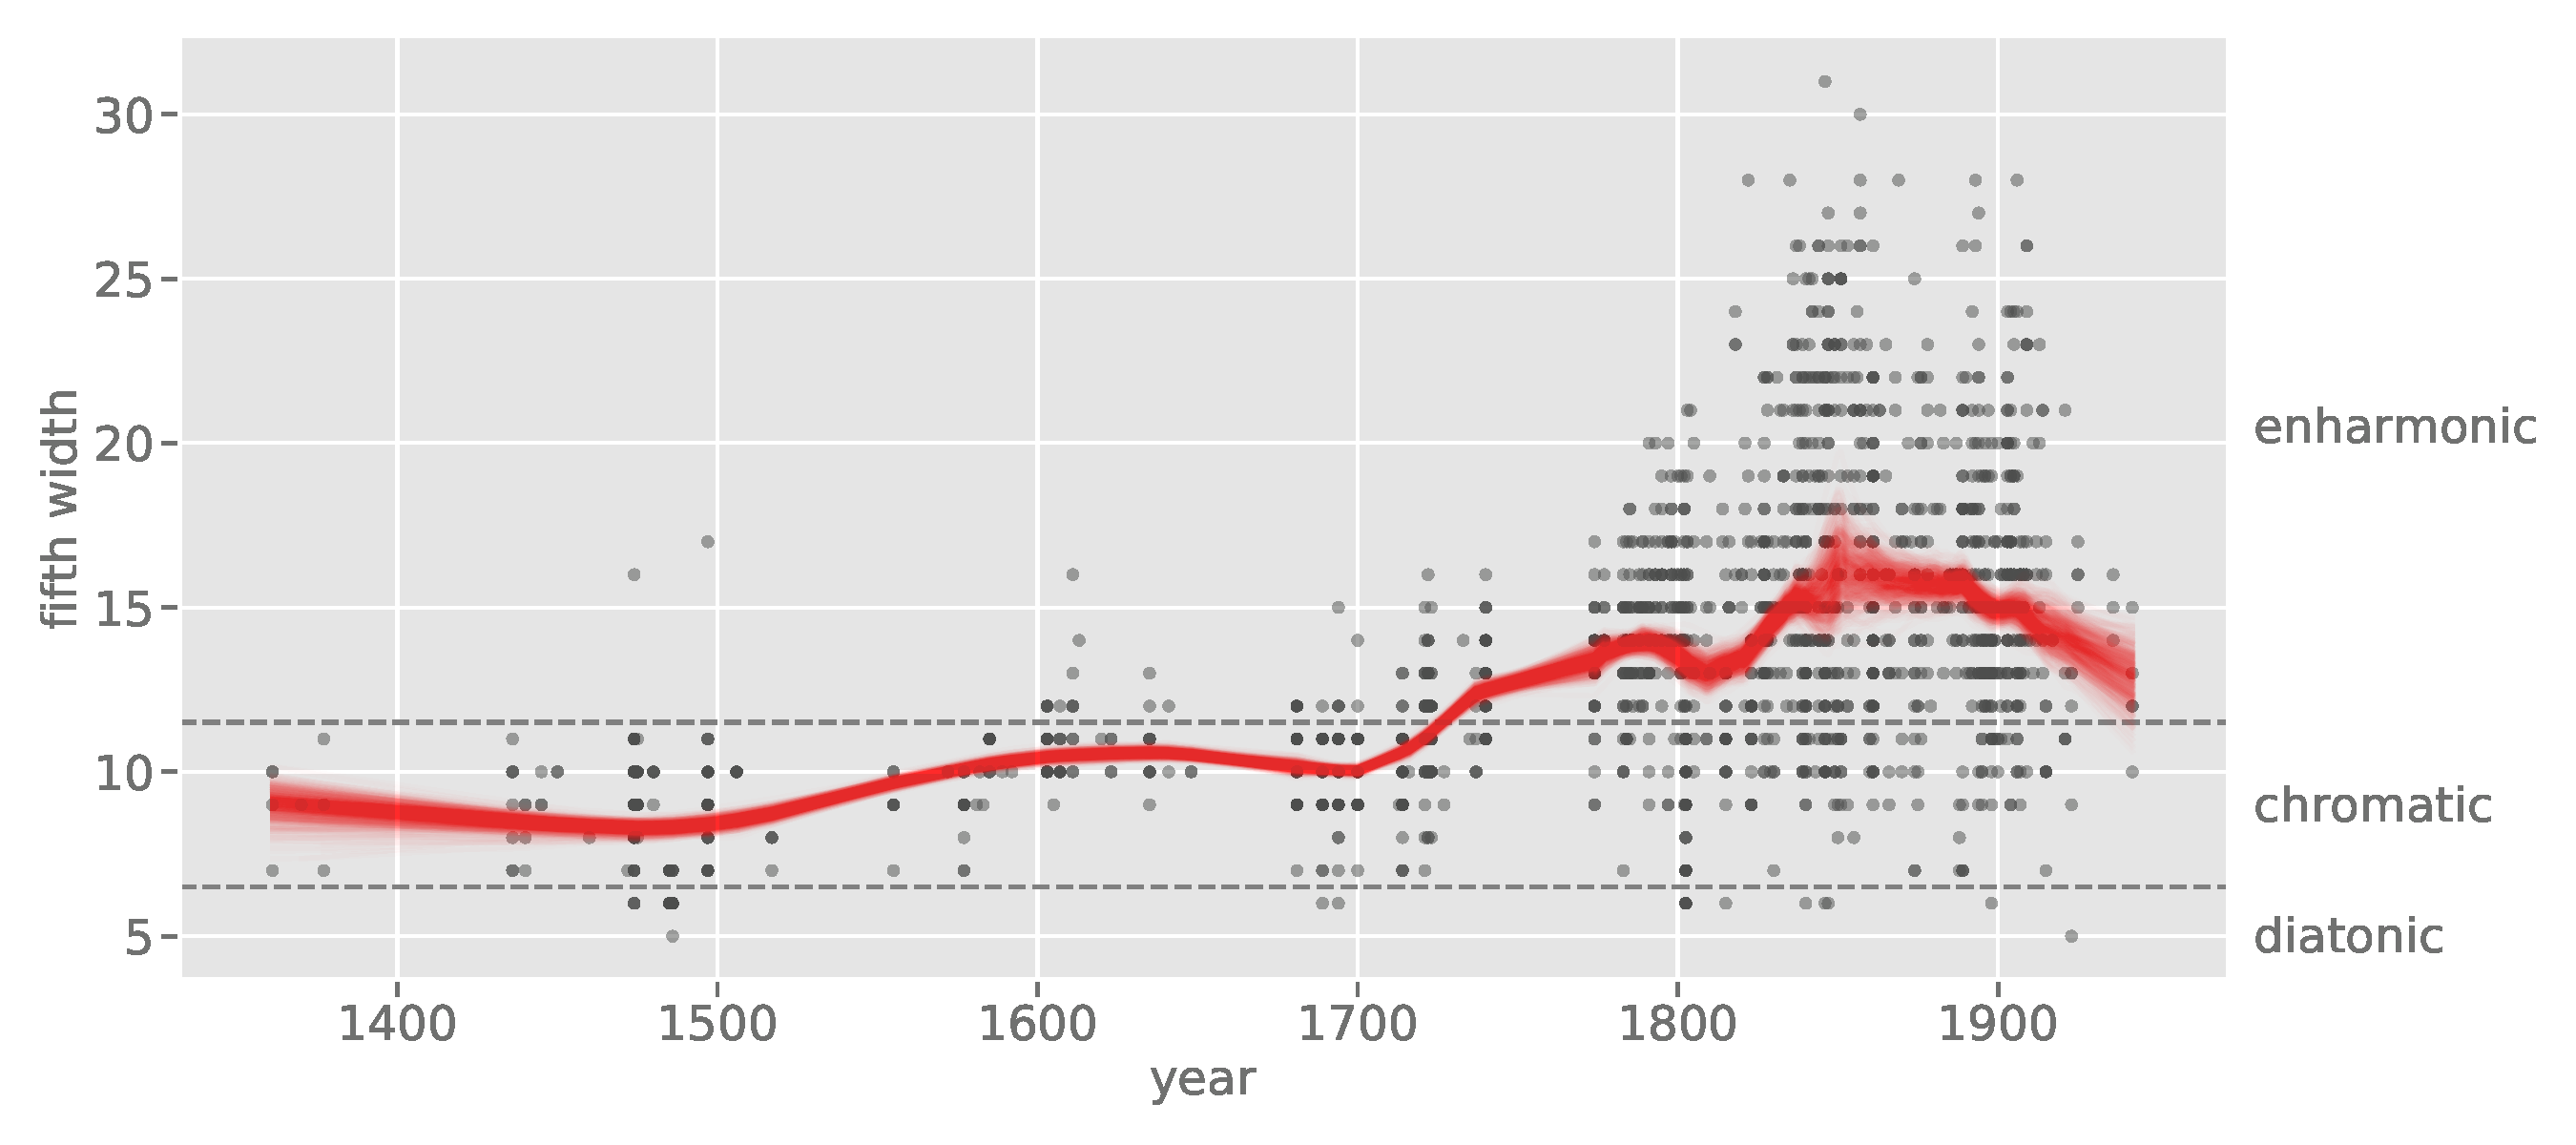
\includegraphics[width=\textwidth]{img/fifth_width.pdf}
    \caption{Historical expansion of tonal material on line of fifths.}
    \label{}
  \end{figure}
\end{frame}

\note[itemize]{
\item Dufay: F\#\# instead of g
\item Ockeghem: Cb instead of C\#
}

\subsection{2. Modelling pieces on the \emph{Tonnetz}}

\begin{frame}{\insertsectionhead}

  Line of fifths is fundamental and simple model but does not explain everything.
  \pause

  $\Rightarrow$ Extend approach to more advanced \alert{models of tonal space}

  \pause
  % Modeling of tonal space in the 19th century: Hauptmann, v. Oettingen, Hostinský, Riemann

  \begin{figure}
    \centering
    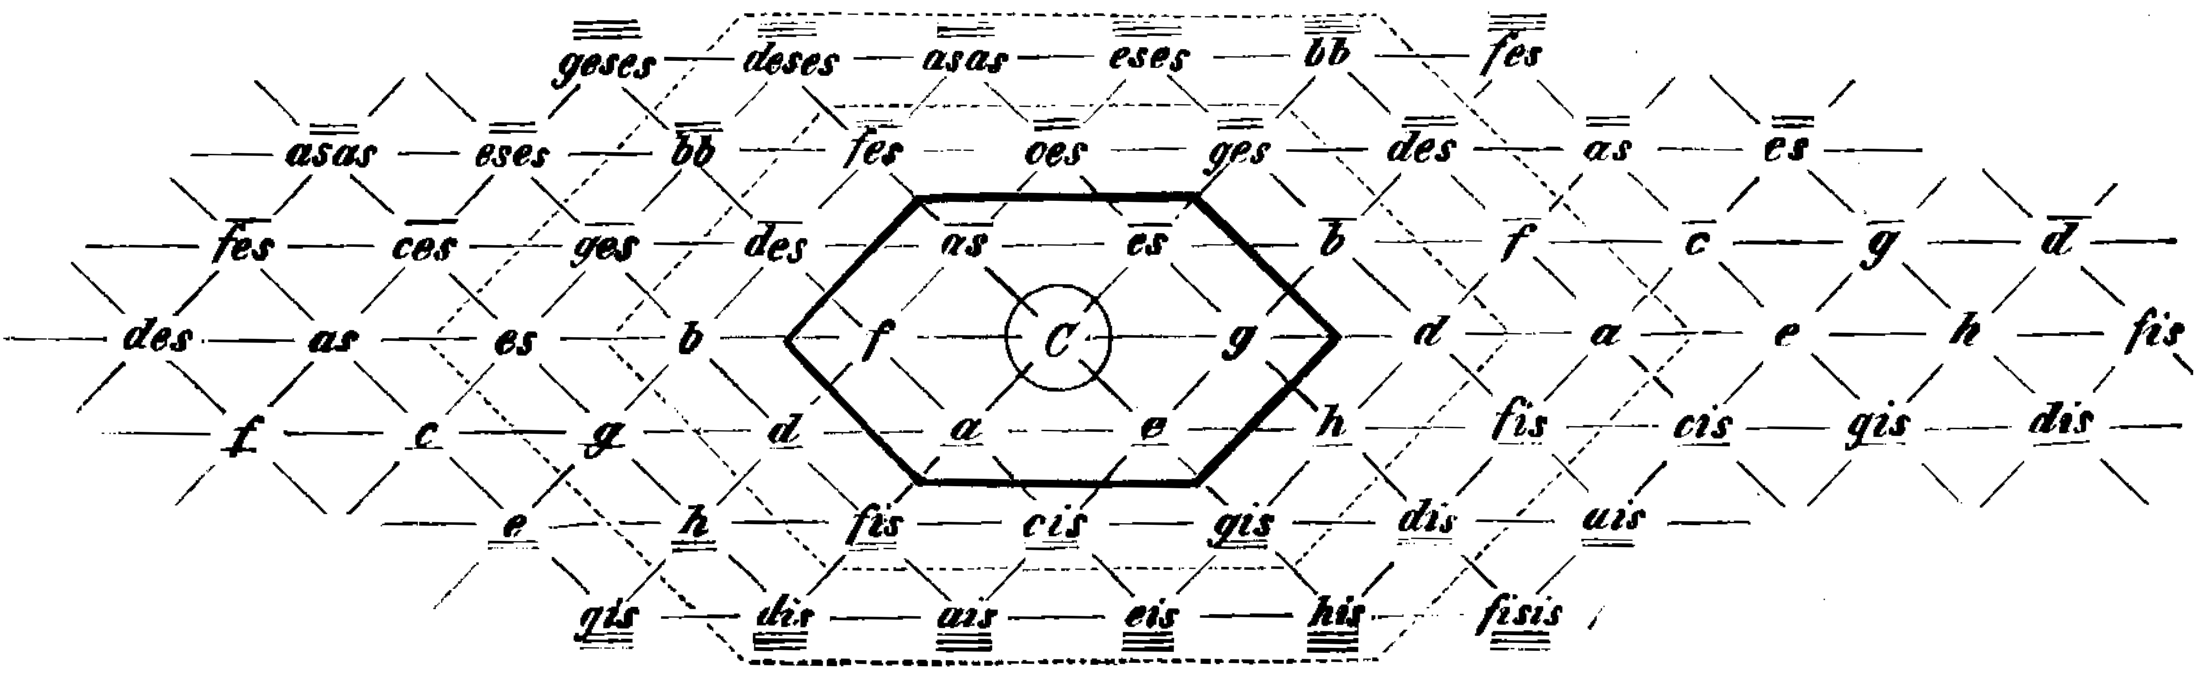
\includegraphics[width=.75\textwidth]{img/hostinsky_tonnetz.png}
    \caption{The \emph{Tonnetz} \citep{Hostinsky1879}.}
    \label{}
  \end{figure}

\end{frame}

\begin{frame}[c]{\insertsectionhead}
  Neo-Riemannian \alert{triadic transformations} on the \emph{Tonnetz}~\citep{Cohn1998}
  \begin{columns}
    \begin{column}{.45\textwidth}
      \begin{itemize}
        \item<2-> \textcolor{epfldark}{parallel ($\mathbf{P}$)}\\ 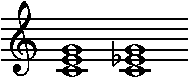
\includegraphics{scores/parallel.pdf}
        \item<3-> \textcolor{canard}{relative ($\mathbf{R}$)}\\ 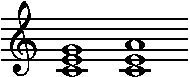
\includegraphics{scores/relative.pdf}
        \item<4-> \textcolor{leman}{leading-tone exchange ($\mathbf{L}$)}\\ 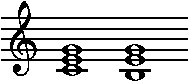
\includegraphics{scores/leading_tone.pdf}
      \end{itemize}

    \end{column}
    %
    \begin{column}{.65\textwidth}
      % TONNETZ WITH ROBERT'S CODE
      %% Figure adapted from https://github.com/DCMLab/TikZ_plot_templates/blob/master/example.tex

  \begin{figure}[c]
    \centering
    % adjust size
    \def\minx{-2}
    \def\maxx{5}
    \def\miny{-2}
    \def\maxy{4}

    % draw hexagons (comment out for not plotting)
    \def\withhex{}
    \newcommand*{\hex}[1]{
      \def\r{0.55}
      \draw[black!7,fill=black!6,visible on=<5->] ($(#1)+(30:\r)$) -- ($(#1)+(90:\r)$) -- ($(#1)+(150:\r)$)  -- ($(#1)+(210:\r)$) -- ($(#1)+(270:\r)$) -- ($(#1)+(330:\r)$) -- cycle;
    }

    \newcommand*{\xy}[2]{
      \pgfmathsetmacro{\x}{#1+cos(60)*#2}
      \pgfmathsetmacro{\y}{sin(60)*#2}
    }
    \newcommand*{\xycoord}[2]{($#1*(1,0)+#2*(60:1)$)}
    \newcommand*{\xycoordcenterbelow}[2]{(${#1+0.333}*(1,0)+{#2+0.333-1}*(60:1)$)}
    \newcommand*{\xycoordcenterabove}[2]{(${#1-0.333}*(1,0)+{#2+0.666}*(60:1)$)}

    \def\r{0.55}
    \tikzstyle{tone}=[circle, draw, fill=white, minimum size=2.5em, thick]
    \scalebox{0.6}{
    \begin{tikzpicture}[scale=2, every path/.style={thick}]
      % create the basic grid
      \foreach \x in {-10,...,10} {
        \foreach \y in {-10,...,10} {
          \pgfmathsetmacro{\xx}{\x+cos(60)*mod(\y+100,2)}
          \pgfmathsetmacro{\yy}{sin(60)*\y}
          \ifthenelse{\x>\minx\AND\x<\maxx\AND\y>\miny\AND\y<\maxy}{
            \ifdefined\withhex\hex{\xx,\yy}\fi
            \coordinate (n_\x_\y) at (\xx,\yy);
            \pgfmathsetmacro{\xMOne}{int(\x-1)}
            \pgfmathsetmacro{\yMOne}{int(\y-1)}
            \pgfmathsetmacro{\yPOne}{int(\y+1)}
            \pgfmathsetmacro{\xxMOne}{\xMOne+cos(60)*mod(\yMOne+100,2)}
            \pgfmathsetmacro{\yyMOne}{sin(60)*\yMOne}
            \pgfmathsetmacro{\yyPOne}{sin(60)*\yPOne}
            \pgfmathsetmacro{\iseven}{int(mod(\y+100,2))}
            \ifthenelse{\xMOne>\minx\AND\xMOne<\maxx}{
              \draw (n_\x_\y) -- (n_\xMOne_\y);
            }{}
            \ifthenelse{\yMOne>\miny\AND\yMOne<\maxy}{
              \draw (n_\x_\y) -- (n_\x_\yMOne);
            }{}
            \ifthenelse{\xMOne>\minx\AND\xMOne<\maxx\AND\yMOne>\miny\AND\yMOne<\maxy}{
              \ifthenelse{\iseven=0}{
                \draw (n_\x_\y) -- (n_\xMOne_\yMOne);
              }{}
            }{}
            \ifthenelse{\xMOne>\minx\AND\xMOne<\maxx\AND\yPOne>\miny\AND\yPOne<\maxy}{
              \ifthenelse{\iseven=0}{
                \draw (n_\x_\y) -- (n_\xMOne_\yPOne);
              }{}
            }{}
          }{}
        }
      }
      % coloured areas
      % \draw[fill=epflred, opacity=0.3] \xycoord{0}{0} -- \xycoord{2}{0} -- \xycoord{2}{1} -- \xycoord{0}{1} -- cycle;
      \draw[fill=epflred, opacity=0.4,visible on=<1->] \xycoord{0}{0} -- \xycoord{1}{0} -- \xycoord{0}{1} -- cycle; % C major
      \draw[fill=epflred, opacity=0.2,visible on=<2->] \xycoord{0}{0} -- \xycoord{1}{0} -- \xycoord{1}{-1} -- cycle; % C minor
      \draw[fill=epflred, opacity=0.2,visible on=<3->] \xycoord{0}{0} -- \xycoord{0}{1} -- \xycoord{-1}{1} -- cycle; % A minor
      \draw[fill=epflred, opacity=0.2,visible on=<4->] \xycoord{1}{0} -- \xycoord{1}{1} -- \xycoord{0}{1} -- cycle; % E minor


      % create tone names
      \foreach \nodename\name/\fifths/\thirds in {
        A+/{A$\sharp$}/-2/3, E+/{E$\sharp$}/-1/3, B+/{B$\sharp$}/0/3, F++/{F$\sharp\sharp$}/1/3, C++/{C$\sharp\sharp$}/2/3, G++/{G$\sharp\sharp$}/3/3,
        F+/{F$\sharp$}/-2/2, C+/{C$\sharp$}/-1/2, G+/{G$\sharp$}/0/2, D+/{D$\sharp$}/1/2, A+/{A$\sharp$}/2/2, E+/{E$\sharp$}/3/2,
        A/A/-1/1, E/E/0/1, B/B/1/1, F+/{F$\sharp$}/2/1, C+/{C$\sharp$}/3/1, G+/{G$\sharp$}/4/1,
        F/F/-1/0, C/C/0/0, G/G/1/0, D/D/2/0, A/A/3/0, E/E/4/0,
        A-/{A$\flat$}/0/-1, E-/{E$\flat$}/1/-1, B-/{B$\flat$}/2/-1, F/F/3/-1, C/C/4/-1, G/G/5/-1
      } {
        \node[tone] (\nodename) at \xycoord{\fifths}{\thirds} {\name};
      }
      % draw some arrows
      % \draw[->, >=stealth, shorten >= 1.5em, shorten <= 1.5em, line width=3pt, epflred] \xycoord{0}{0} -- \xycoord{1}{1};
      % \draw[->, >=stealth, line width=3pt, violet] \xycoordcenterbelow{1}{1} -- \xycoordcenterabove{3}{0};
      % \draw[->, >=stealth, line width=3pt, green] \xycoord{0.5}{1.5} -- \xycoord{1.5}{1.5};
      % \draw[->, >=stealth, line width=3pt, blue] \xycoord{-0.75}{2.5} -- \xycoord{1.25}{2.5};
      \draw[->, >=stealth, line width=2pt, epfldark,visible on=<2->] \xycoordcenterbelow{0}{1} -- \xycoordcenterabove{1}{-1} node [pos=.25, right] {$\mathbf{P}$}; % parallel
      \draw[->, >=stealth, line width=2pt, canard,visible on=<3->] \xycoordcenterbelow{0}{1} -- \xycoordcenterabove{0}{0} node [pos=.3, below] {$\mathbf{R}$}; % relative
      \draw[->, >=stealth, line width=2pt, leman,visible on=<4->] \xycoordcenterbelow{0}{1} -- \xycoordcenterabove{1}{0} node [pos=.2, above] {$\mathbf{L}$}; % leading-tone
    \end{tikzpicture}
    }
    \caption{The \emph{Tonnetz}.}
\end{figure}

    \end{column}
  \end{columns}
\end{frame}

\note[itemize]{
\small
\item While Neo-Riemannian transformations on the \emph{Tonnetz} are a useful analytical
  technique for a great deal of music, it has an obvious limitation:
\item It requires that the music under consideration is triadic.
\item There are a number of approaches trying to extend the classical paradigm, e.g.
  by also considering seventh chords.
\item But as an analyst, one can not know in advance which kinds of sonorities one will
  encounter with a new, maybe unknown piece.
\item Fortunately, there is a way out of this dilemma.
\item We can consider the \emph{Dual Tonnetz} in which not triads but the notes are in the focus.
\item This hexagonal reprentation allows us to visualise notes as they occur in a piece or in a section thereof,
  and to compare pieces with one another.
\item This approach is particularly relevant since we want to understand the historical development of tonality.
}

\begin{frame}[fragile]{\insertsectionhead}

  \begin{columns}
    \begin{column}{.5\linewidth}
      % The \emph{dual Tonnetz}

      \begin{itemize}
        \item<2-> \alert{diatonic} $\pm$ P5\\
        \vspace{1em}
          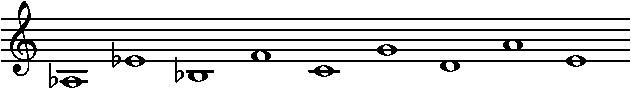
\includegraphics[width=\linewidth]{scores/diatonic.pdf}
        \item<3-> \alert{octatonic} $\pm$ m3, $\pm$ P5\\
        \vspace{1em}
          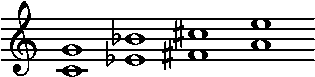
\includegraphics[width=.55\linewidth]{scores/octatonic.pdf}
        \item<4-> \alert{hexatonic} $\pm$ M3, $\pm$ P5\\
        \vspace{1em}
          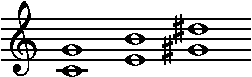
\includegraphics[width=.45\linewidth]{scores/hexatonic.pdf}
      \end{itemize}
    \end{column}
    %
    \begin{column}{.5\linewidth}

    \begin{figure}[tbp]
    \centering
    \newcommand*{\hex}[1]{
      \def\r{0.55}
      \draw[black!6,fill=black!4] ($(#1)+(30:\r)$) -- ($(#1)+(90:\r)$) -- ($(#1)+(150:\r)$)  -- ($(#1)+(210:\r)$) -- ($(#1)+(270:\r)$) -- ($(#1)+(330:\r)$) -- cycle;
    }
    \begin{tikzpicture}[scale=1.7]
      % hexagon
      \hex{0,0}
      % notes
      \foreach \a/\l/\i/\p in {
        0/G/{$+$P5}/below,
        -60/{E$\flat$}/{$+$m3}/below,
        -120/{A$\flat$}/{$-$M3}/above,
        -180/F/{$-$P5}/above,
        -240/A/{$-$m3}/above,
        -300/E/{$+$M3}/below,
        1000/// % hack to avoid weird tikz label problem
      } {
        \ifthenelse{\a=1000}{}{
          \hex{\a:1}
          \draw (\a:0.15) edge[->,>=stealth,line width=1,shorten >=.5em] node[\p ,sloped,fill=white,fill opacity=0,text opacity=1] {\scalebox{0.8}{\i}} (\a:0.85);
          \node [circle,draw,black, fill=white, minimum size=2em] at (\a:1) {\l};
        }
      }
      % center
      \node [circle,draw,black, fill=white, minimum size=2em] at (0,0) {C};
    \end{tikzpicture}
    % \caption{Primary intervals with respect to C.}\label{fig:primary_intervals}
  \end{figure}
\end{column}
\end{columns}
\end{frame}

\begin{frame}{\insertsectionhead}

  \begin{columns}
    \begin{column}{.33\linewidth}
      \centering
      \alert{diatonic}

      \vspace{1em}

      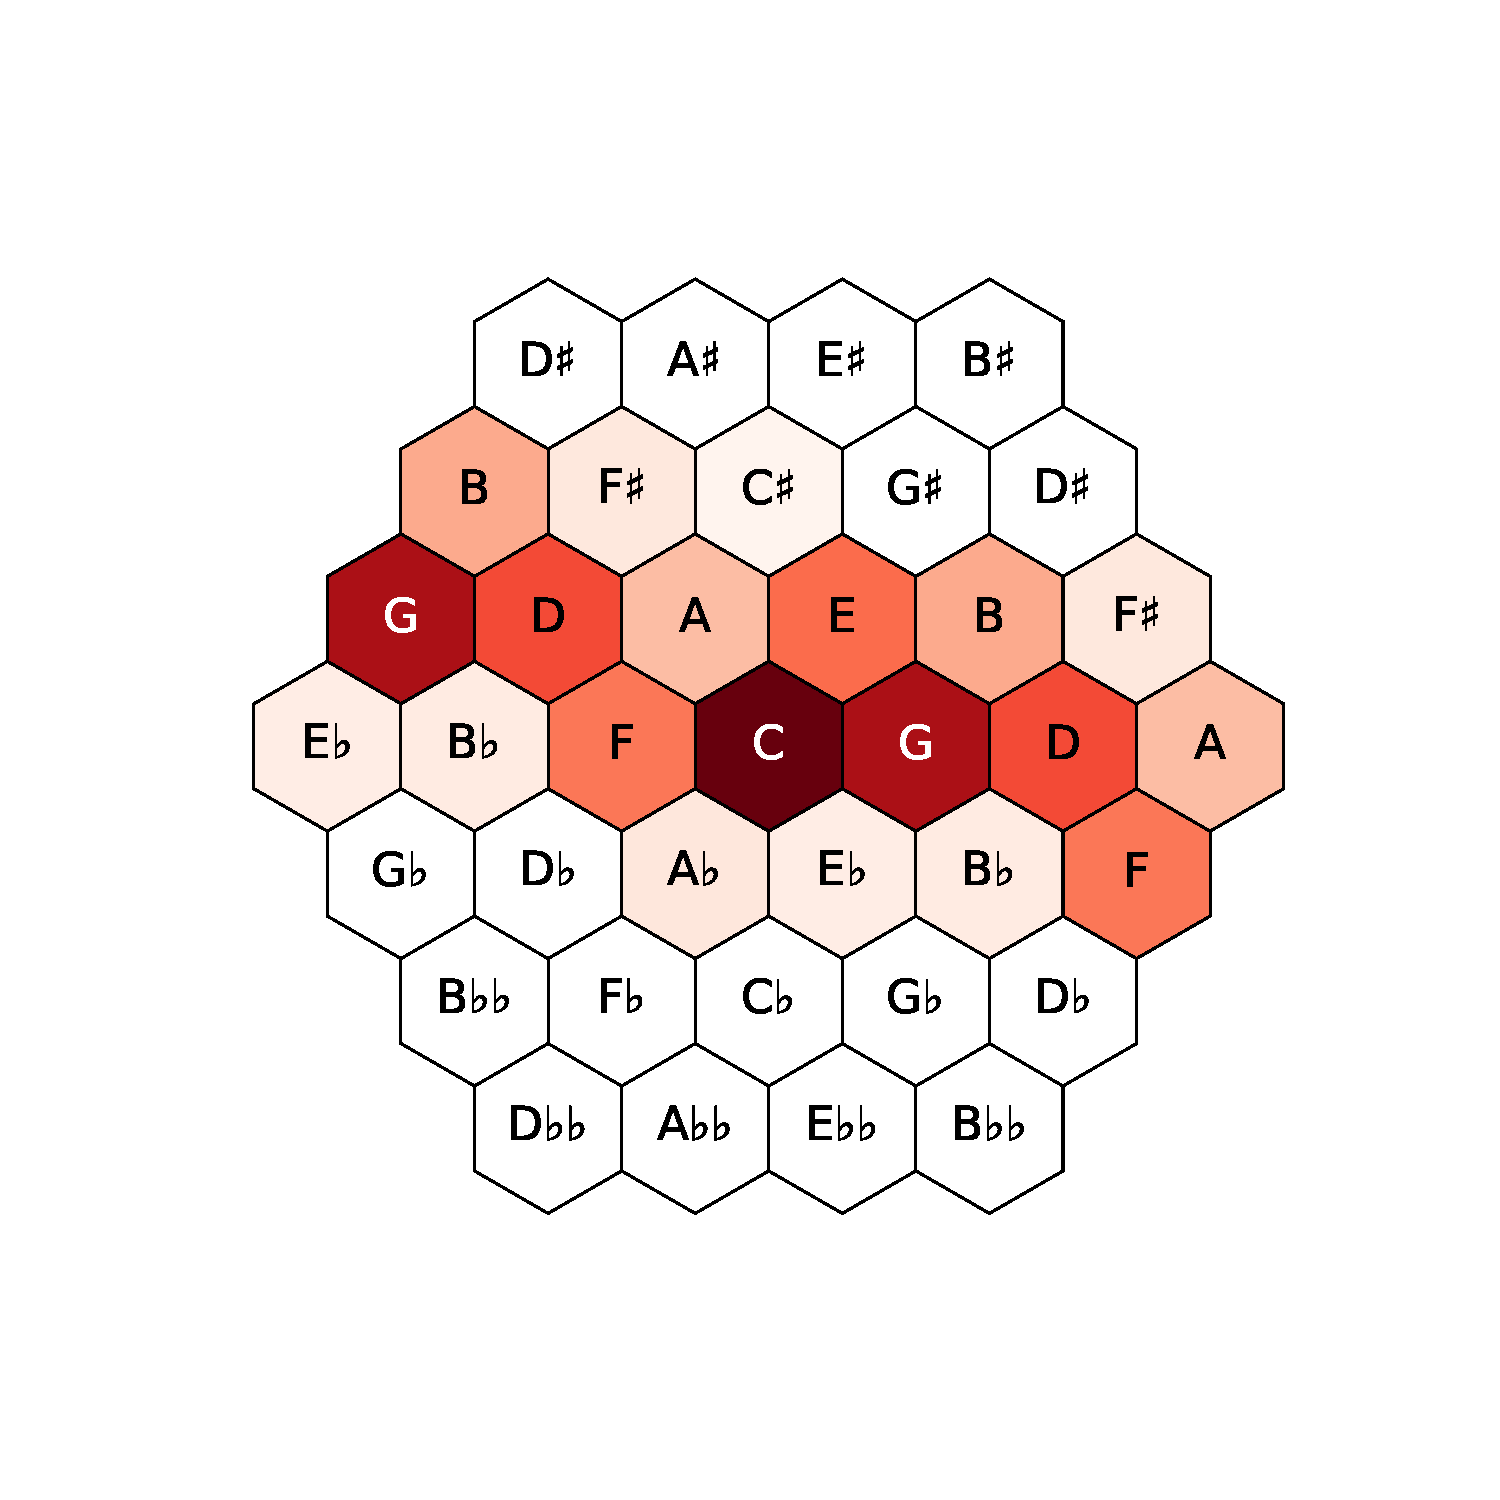
\includegraphics[trim=0 100 0 100, clip, width=\linewidth]{img/bach.pdf}
      Bach, \emph{Prelude in C major}, BWV~846 (1722).
    \end{column}
    %
    \pause
    %
    \begin{column}{.33\linewidth}
      \centering
      \alert{hexatonic}

      \vspace{1em}

      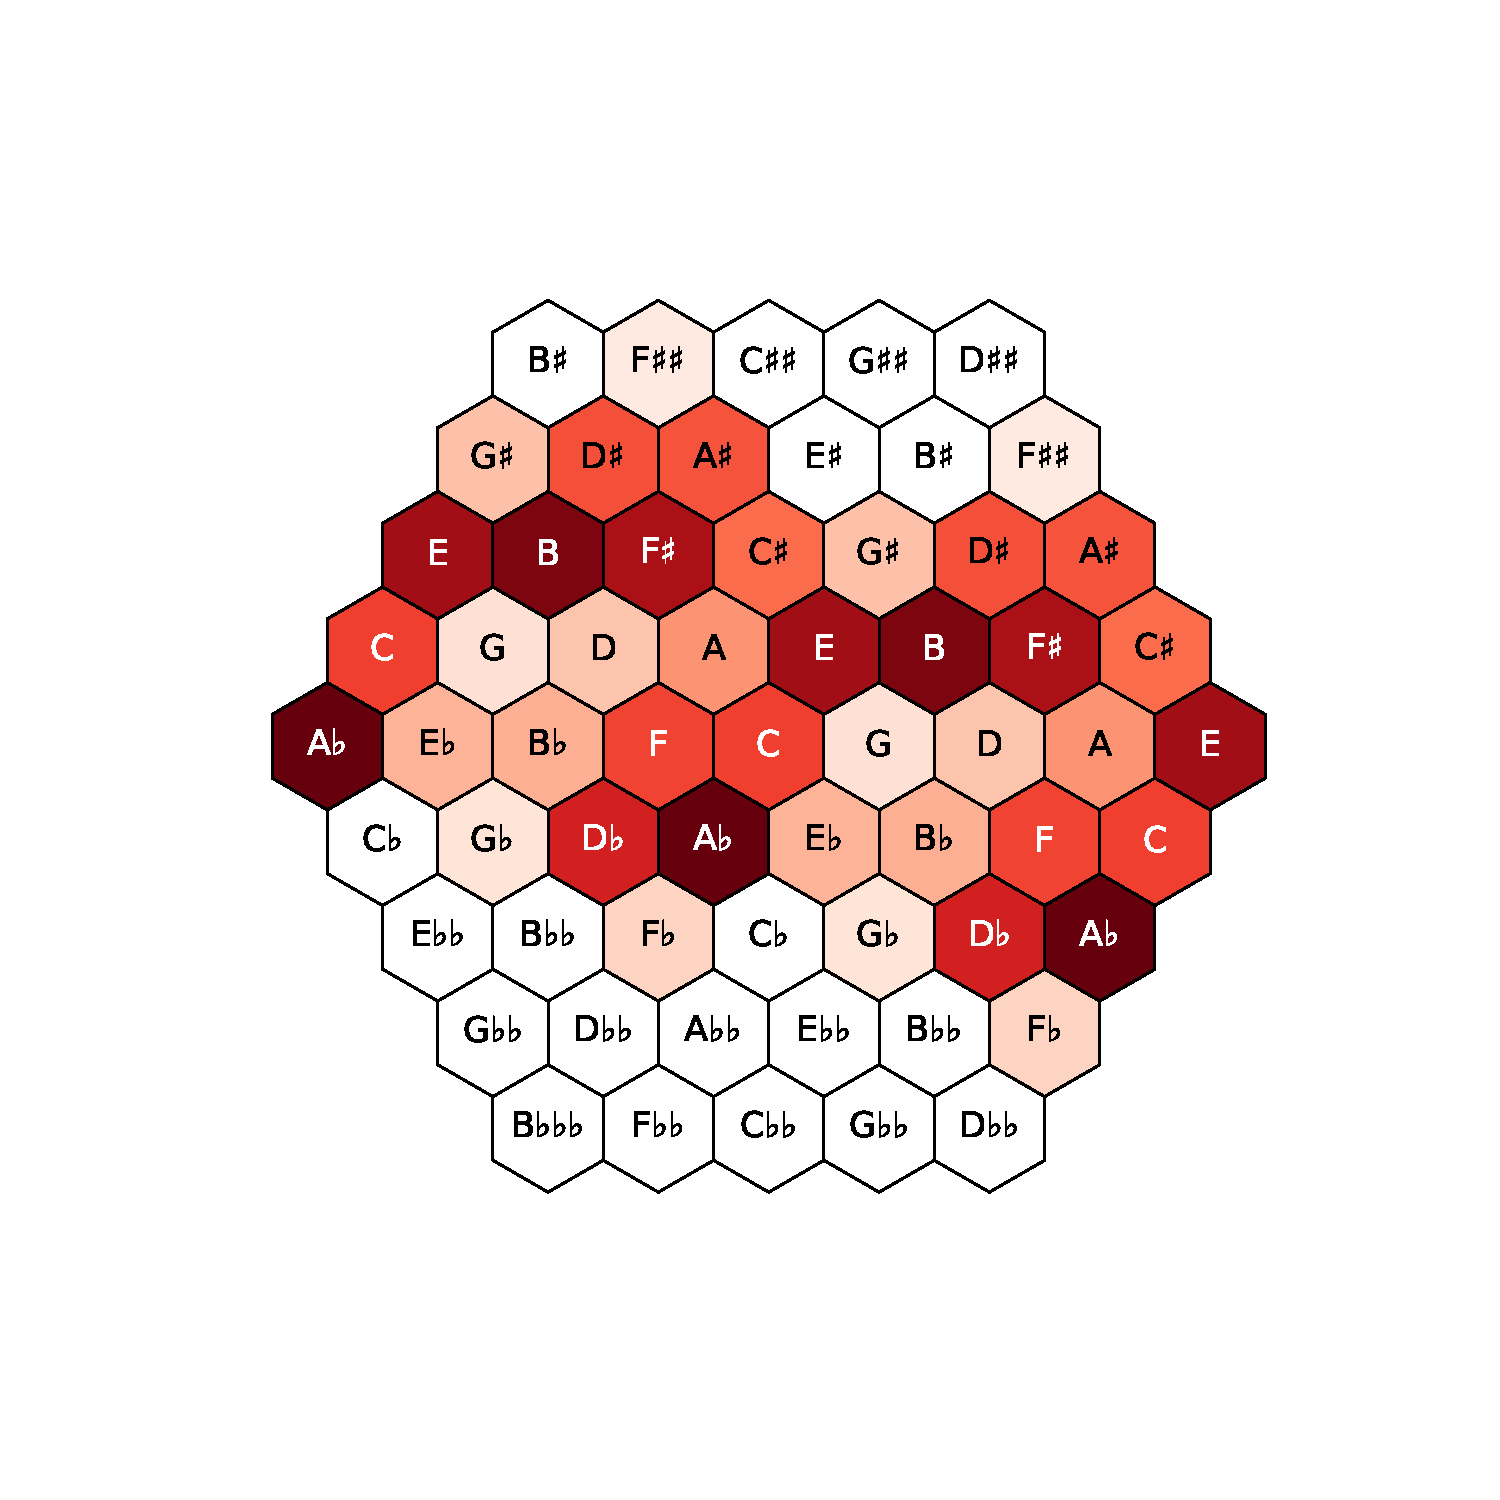
\includegraphics[trim=0 100 0 100, clip, width=\linewidth]{img/liszt.pdf}
      Liszt, \emph{Lugubre gondola I}, S.~200/1~(1882).
    \end{column}
    %
    \pause
    %
    \begin{column}{.33\linewidth}
      \centering
      \alert{octatonic}

      \vspace{1em}

      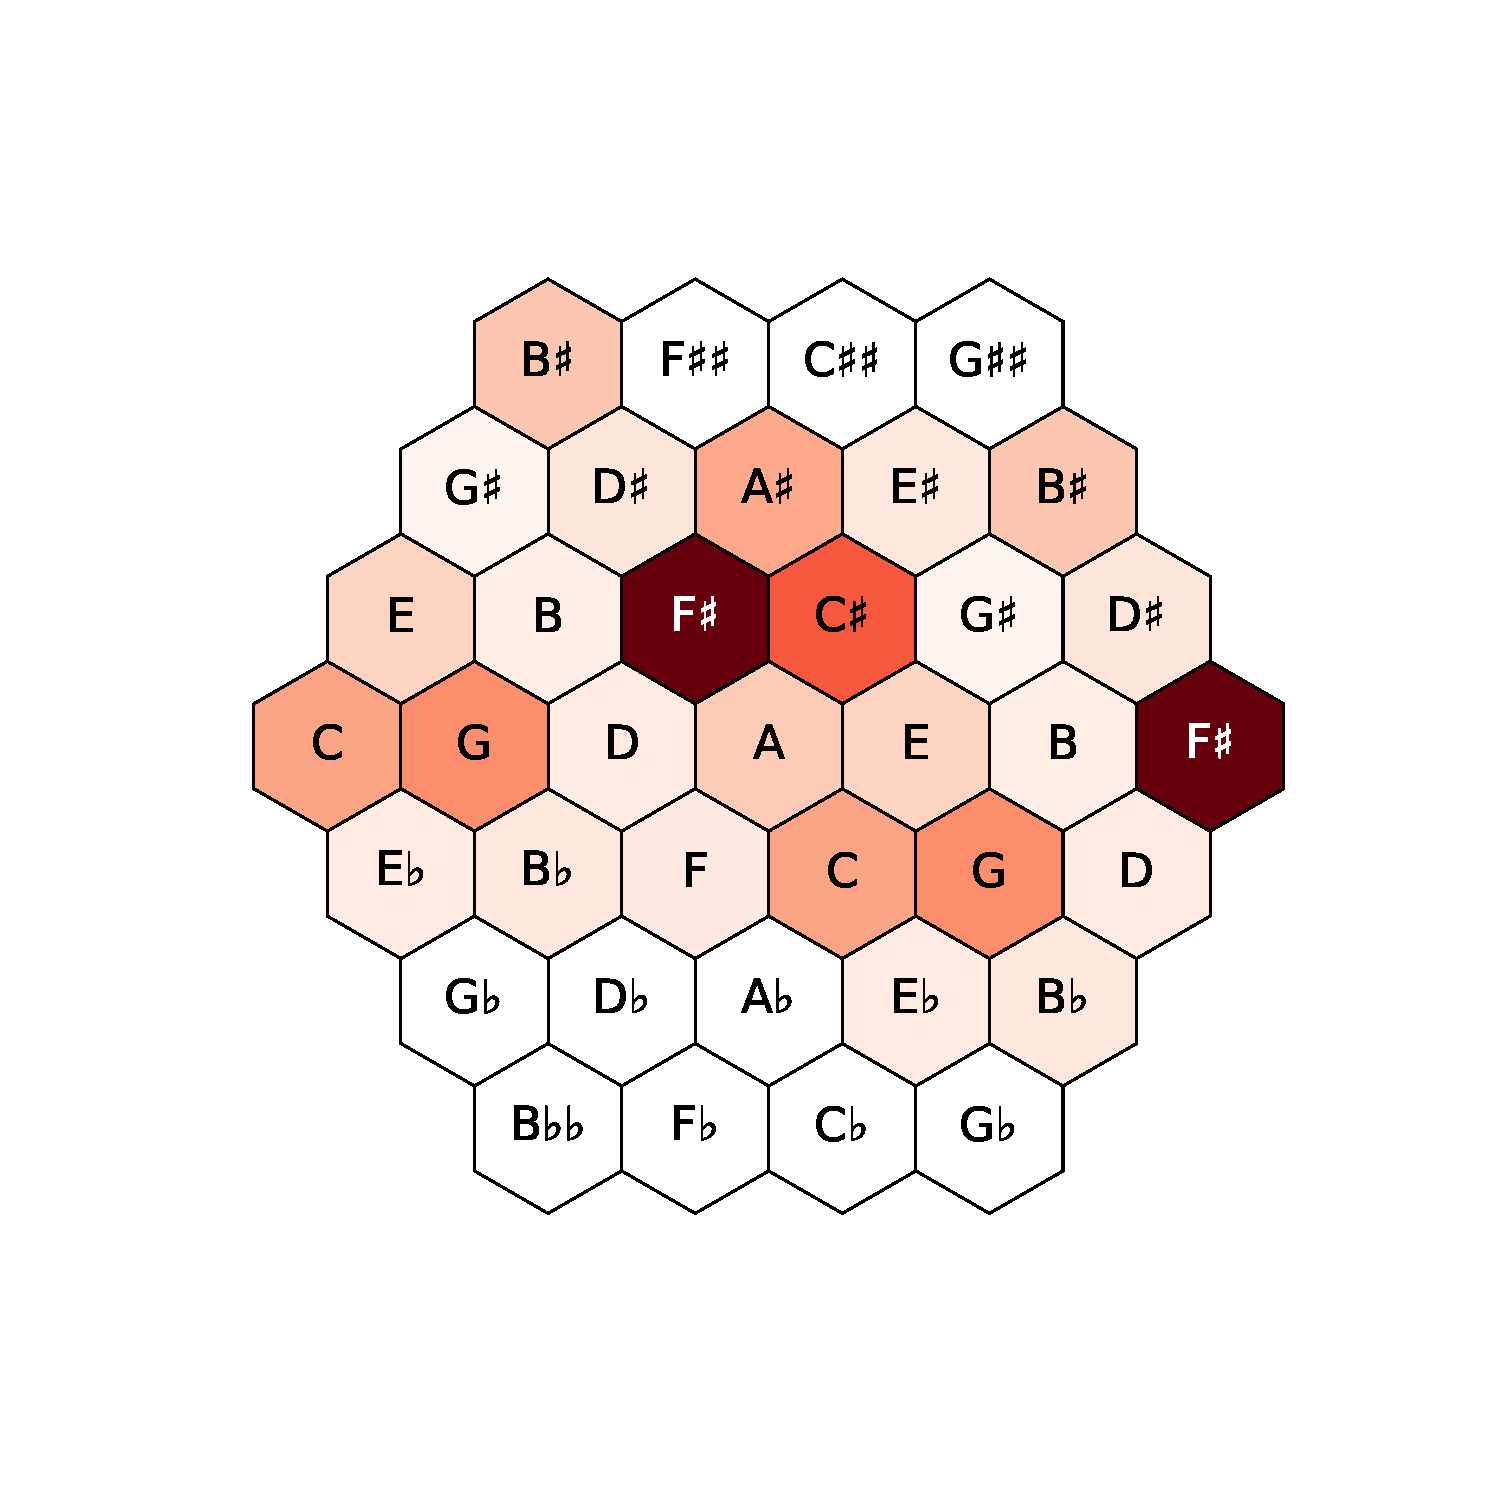
\includegraphics[trim=0 130 0 100, clip, width=\linewidth]{img/scriabin.pdf}
      Scriabin, \emph{Prelude}, op.~74/2~(1914).
    \end{column}
  \end{columns}

  % \begin{figure}
  %   \centering
  %   \begin{subfigure}[t]{.3\textwidth}
  %     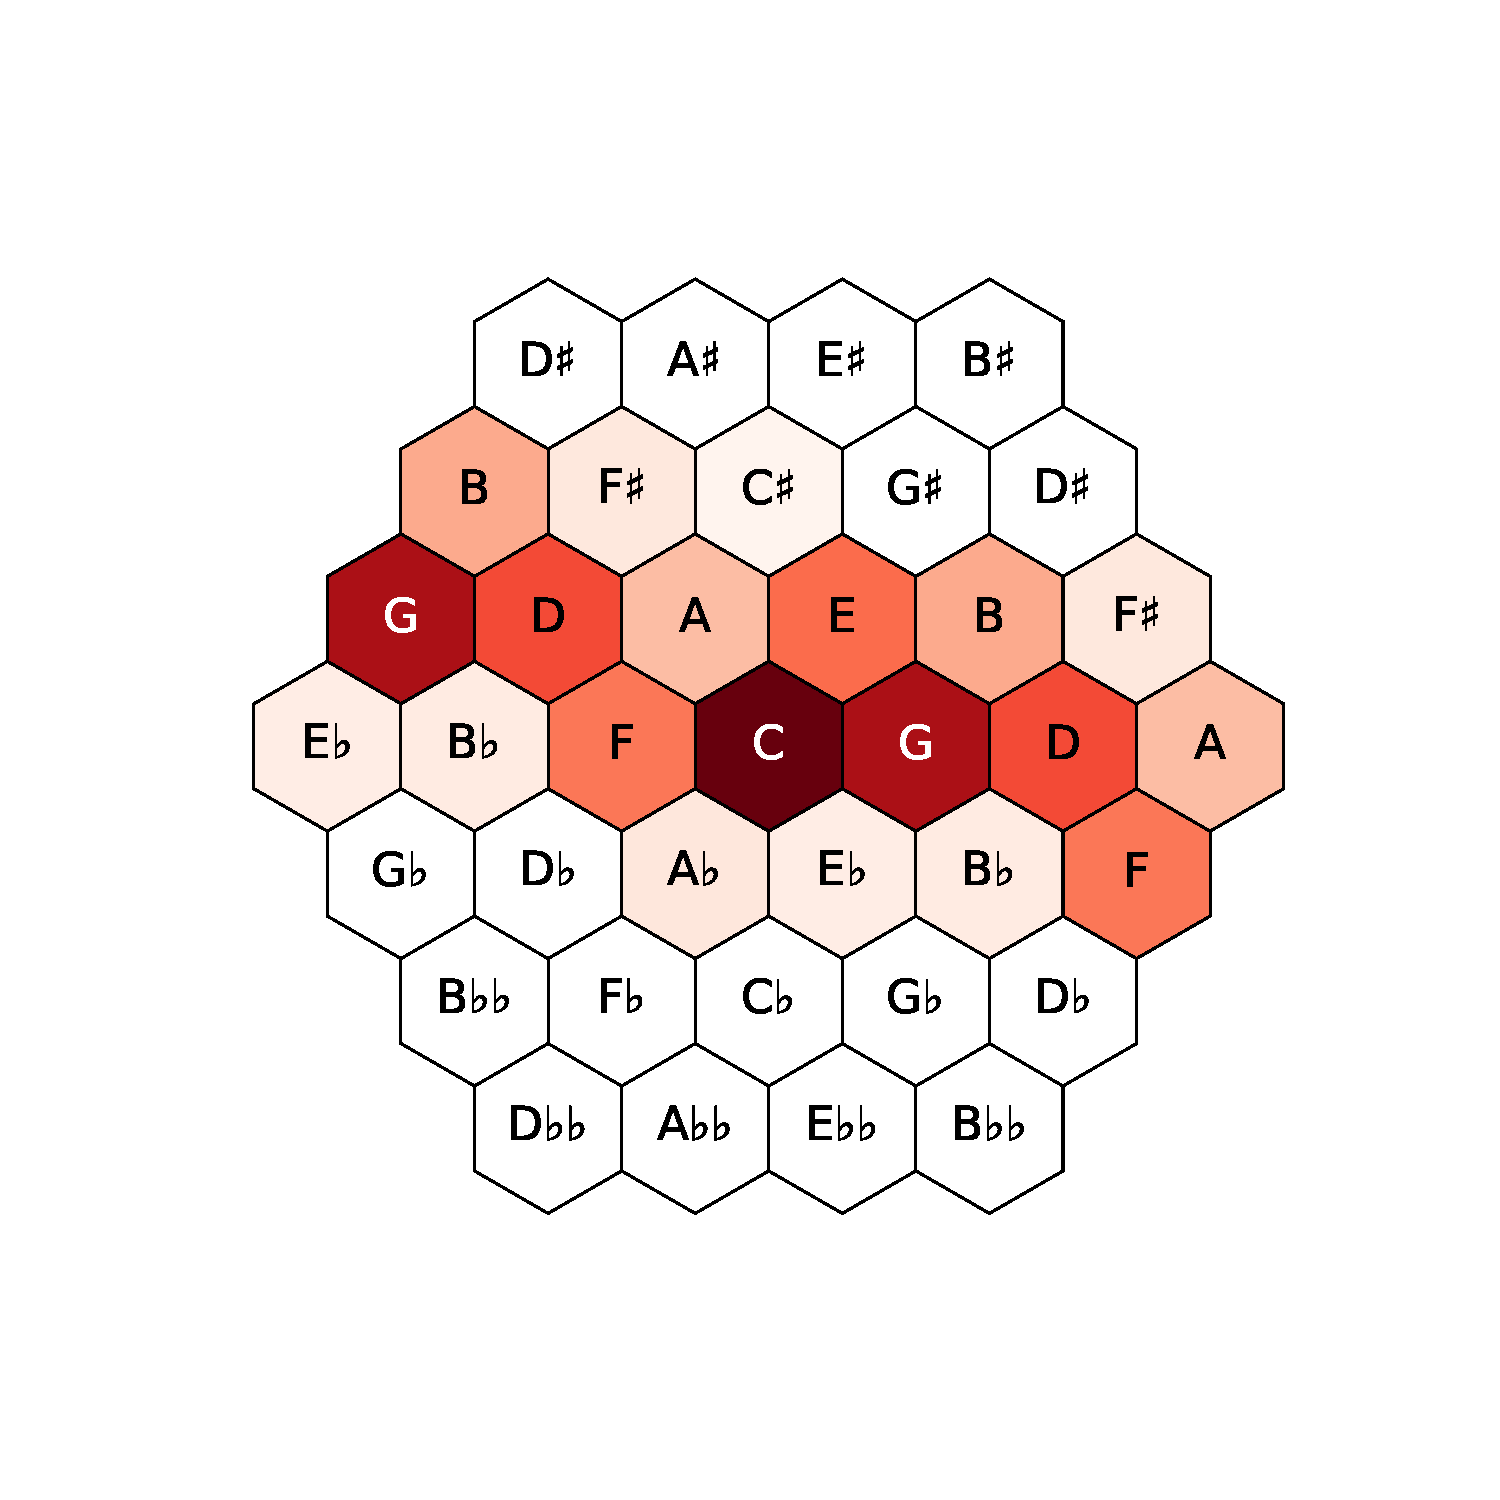
\includegraphics[width=\linewidth]{img/bach.pdf}
  %     \subcaption*{Bach, \emph{Prelude in C major}, WTC I, (1722).}
  %   \end{subfigure}
  %   \hfill
  %   \begin{subfigure}[t]{.3\textwidth}
  %
  %   \end{subfigure}
  %   \hfill
  %   \begin{subfigure}[t]{.3\textwidth}
  %
  %   \end{subfigure}
  %   \caption{Historical differences in note distributions.}
  % \end{figure}
\end{frame}

\note[itemize]{
\item Most importantly, this approach does not need a reduction to triads prior to analysis, since the notes can
  be taken from the score as they are written.
\item However, as in the case of the classical \emph{Tonnetz}, we consider octave related notes as equivalent.
}

\begin{frame}{\insertsectionhead}
  Computational model assumptions
  \begin{enumerate}[\color{epflred}1.]
    \item all notes are related to a \alert{tonal center}
    \item relations are given by (combinations of) \alert{intervals} on the \emph{Tonnetz}
  \end{enumerate}
\end{frame}

\begin{frame}{\insertsectionhead}
  \begin{enumerate}[\color{epflred}1.]
    \item \textbf{Initial computational model and analysis}\\\citet{Moss2019a}.~\citetitle{Moss2019a}.
    \item \textbf{Extensions of model}\\\citet{Lieck2020}.~\citetitle{Lieck2020}.
    \item \textbf{Extensions of analysis}\\\citet{Moss2020b}.~\citetitle{Moss2020b}.
  \end{enumerate}
\end{frame}


\begin{frame}{\insertsectionhead}

  \begin{figure}[h]
    \onslide<1->{
	\begin{subfigure}{0.44\linewidth}
		\centering
		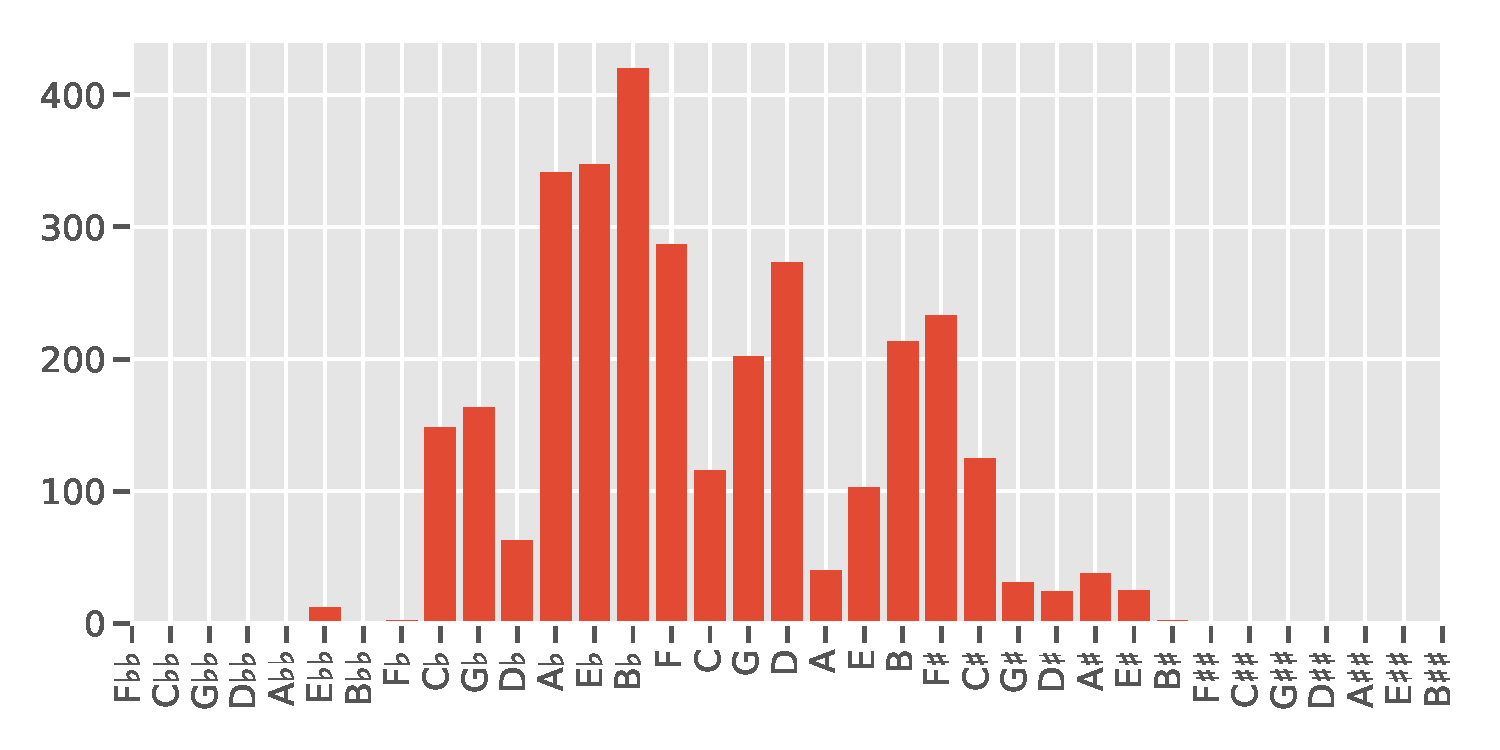
\includegraphics[width=\textwidth]{img/tpc_dists.pdf}
	\end{subfigure}}
  %
  \hfill
  \onslide<2->{
	\begin{subfigure}{0.24\linewidth}
		\centering
		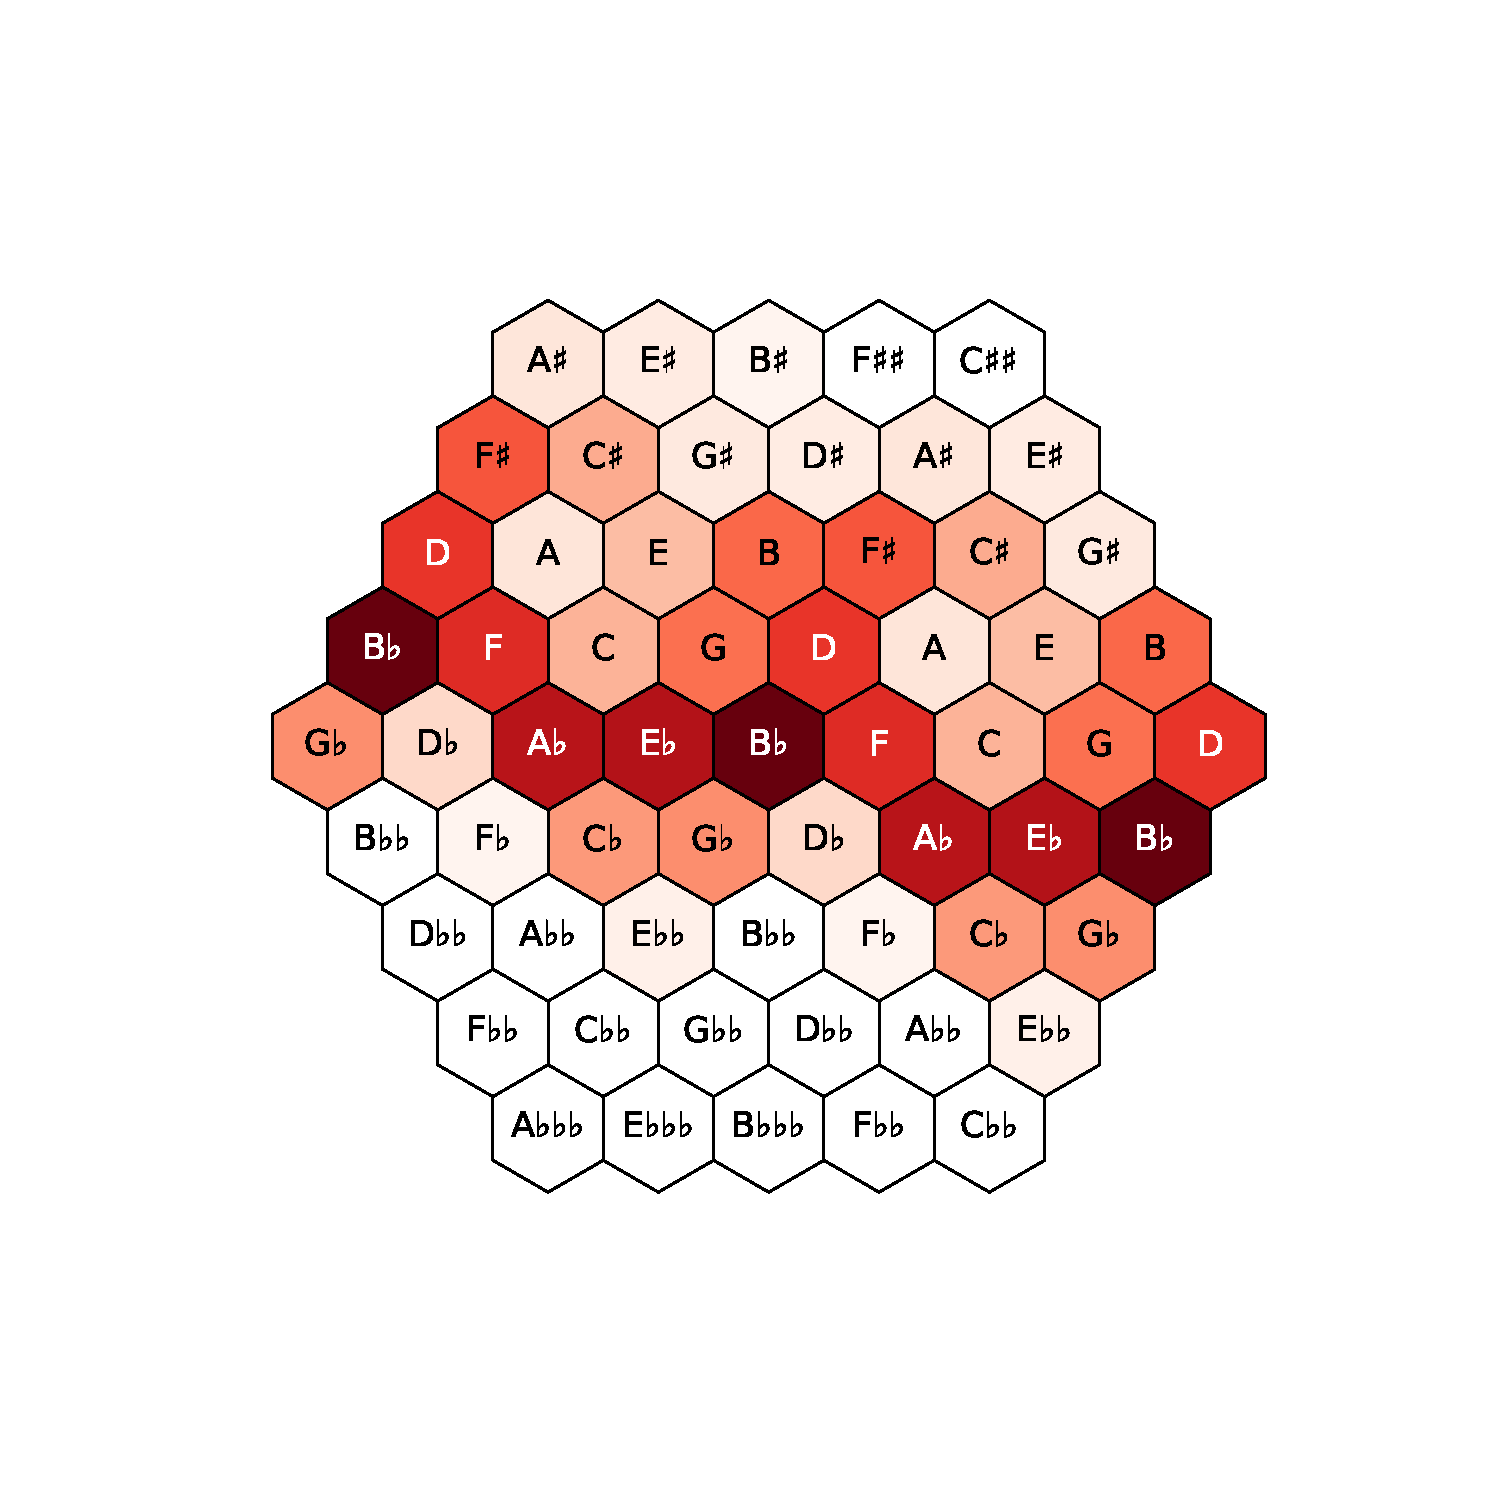
\includegraphics[width=\textwidth, trim=110 140 110 140,clip]{img/Schubert_90_2.pdf}
	\end{subfigure}}
  %
  \hfill
  \onslide<3->{
  \begin{subfigure}{0.29\linewidth}
		\centering
		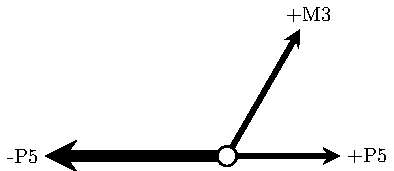
\includegraphics[width=\textwidth]{img/tikz_Schubert_90_2.pdf}
	\end{subfigure}}
	\caption{F. Schubert, \emph{Impromptu}, op. 90/2 in E$\flat$ major.}
	% \label{}
\end{figure}

\onslide<4->{

Model finds six \alert{interval parameters} that best explain the notes in a piece.
\begin{itemize}
  \item only based on \alert{explicit} music-theoretical assumptions $\rightarrow$ criticism
  \item looking at all parameters for all pieces in the corpus shows \alert{historical trends}
\end{itemize}
}

\end{frame}

\begin{frame}
  % \begin{columns}
  %   \begin{column}{.4\textwidth}
  %     \begin{itemize}
  %       \item Computational Model to infer most likely interval usage~\citep{Lieck2020}
  %       \item Perfect fifths are highly relevant throughout history
  %       \item Major and minor third directions are explored abundantly in the 19th century
  %     \end{itemize}
  %   \end{column}
  %   %
  %   \begin{column}{.6\textwidth}
      \begin{figure}
        \centering
        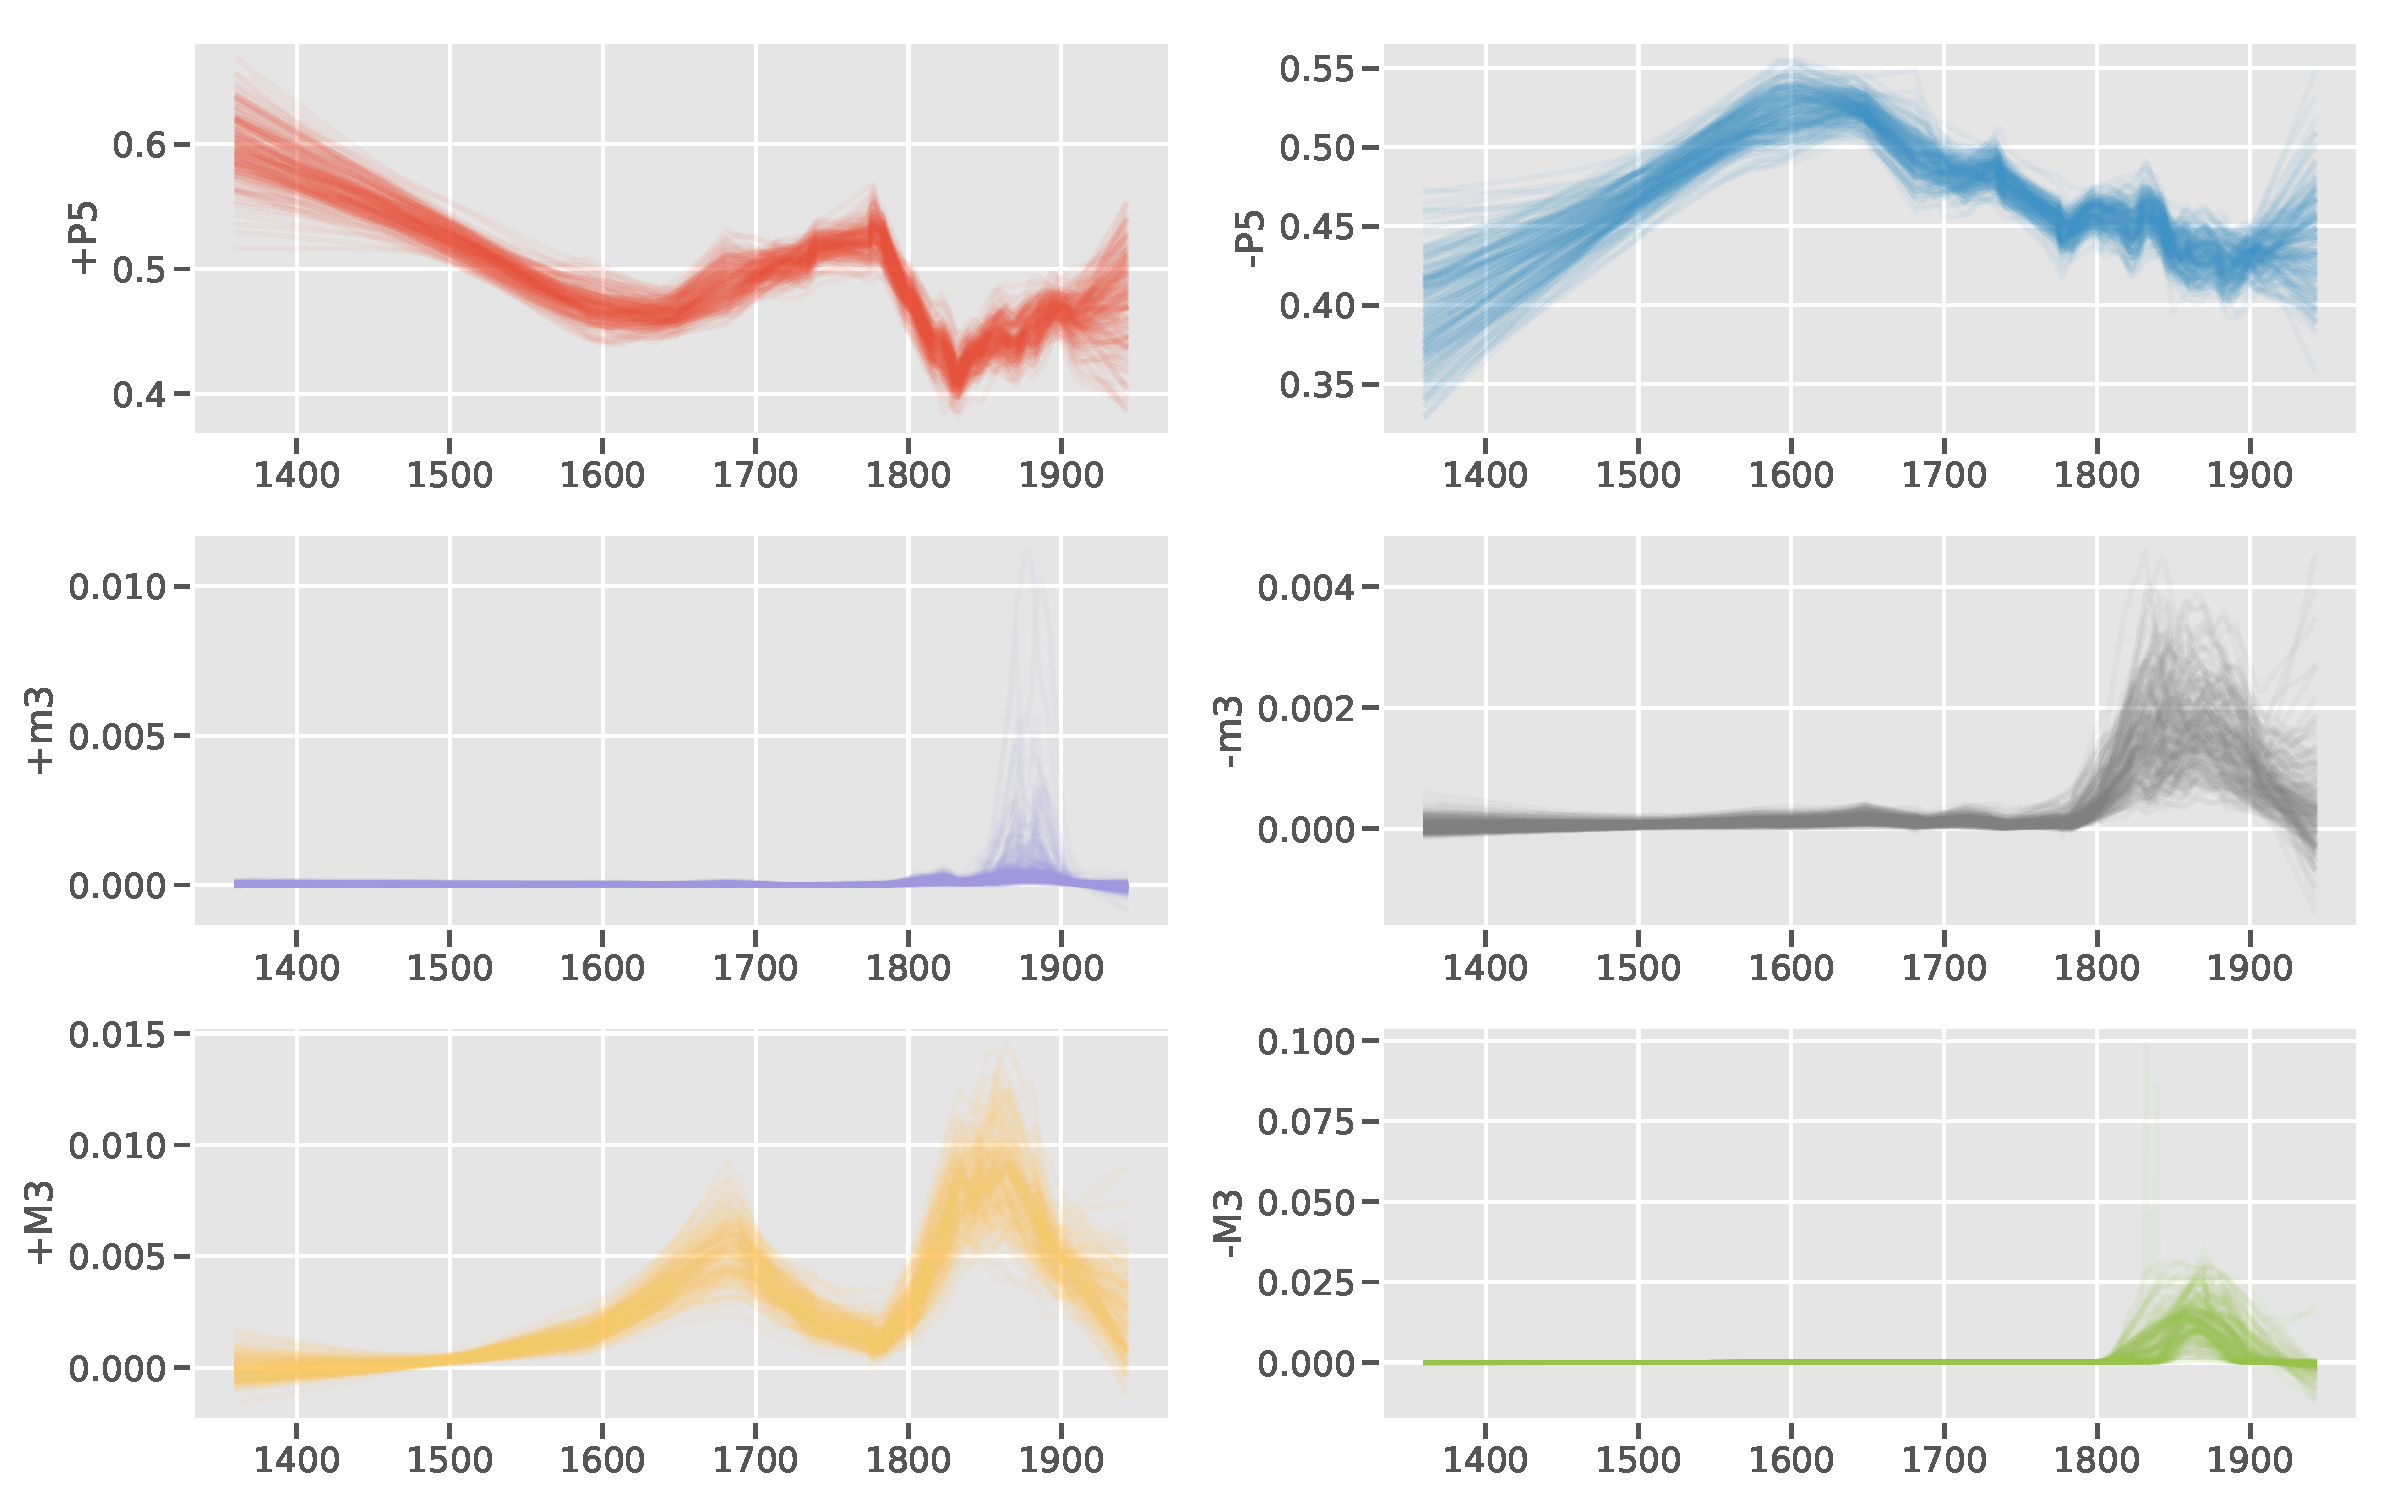
\includegraphics[width=.65\textwidth]{img/bootstrapped_weights.pdf}
        \caption{Historical changes in interval usage on the \emph{Tonnetz}.}
        \label{}
      \end{figure}
  %   \end{column}
  % \end{columns}
\end{frame}

% \begin{frame}{\insertsectionhead}
%   \begin{enumerate}[\color{epflred}1.]
%     \item<1-> model finds \alert{best explanations} for relations between notes
%     \item<2-> only based on \alert{explicit assumptions} of the model $\rightarrow$ criticism
%     \item<3-> corpus studies allow to analyze \alert{changes of tonality} on a large scale
%   \end{enumerate}
% \end{frame}

% \begin{frame}{Summary and Prospects}
%   \begin{enumerate}[\color{epflred}1.]
%     \item \ldots
%     \item \ldots
%     \item Tonality tells only one part of the story. Many other aspects of music are relevant as well,
%     e.g. form, meter, instrumentation, tuning, social contexts, reception, \ldots
%   \end{enumerate}
% \end{frame}
